\documentclass[12pt]{article}
	\usepackage[danish]{babel}
	\usepackage{tabularx}
	\usepackage{varwidth}
	\usepackage{array}
    \usepackage[margin=1in]{geometry}
    \usepackage{amsmath}
    \usepackage[utf8]{inputenc}
    \usepackage{graphicx}
    \usepackage{fancyhdr}
    \usepackage{lastpage}
    \usepackage[T1]{fontenc}
    \usepackage{amssymb}
    \usepackage{listings}
    \usepackage{minted}
    \usepackage[colorinlistoftodos]{todonotes}
    \usepackage{wrapfig}
    \usepackage{subcaption}
    \usepackage{hyperref}
    \usepackage{todonotes}
    \usepackage[final]{pdfpages}
    \usepackage{parskip}
    \usepackage{float}
    \usepackage{adjustbox}
    \usepackage{colortbl}
    \usepackage{color}
    \usepackage{xcolor}
    \definecolor{Gray}{gray}{0.8}
    \definecolor{LightGray}{gray}{0.9}
    \definecolor{WhiteGray}{gray}{0.95}
    
    \pagestyle{fancy}

    \title{Diabetes og Min Sundhedsplatform - Dybdeanalyse}
    \author{Casper Bresdahl whs715\\ Torben Olai Milhøj vrw704\\ Sarah Willumsen zql291\\ Mads Rosenlund Jensen lfh632\\}
    \date{}
    \begin{document}
        \maketitle
        \thispagestyle{empty}
        \cfoot{Page \thepage ~of \pageref{LastPage}}
        %Af en eller anden grund stod der INDHOLD i sidehovedet, disse tre linjer fjerner dette
        \chead{}
        \lhead{}
        \rhead{}
        %Fjerner linjen i sidehovedet
        \renewcommand{\headrulewidth}{0pt}

        \pagestyle{empty}
        {
        	\renewcommand{\thispagestyle}[1]{}
        	\tableofcontents
        }
        \clearpage
        \pagestyle{fancy}
        \newpage
        \setcounter{page}{1}
        	%
%
%
%
%
%
% Er igang med rette i denne i forbindelse med feedback fra Anders
%
%
%
%
%
%
%
%
%
%
%
%
%
%
%
%
%
%
%
%
%
\section{Visioner om den samlede forandring}
I dette afsnit beskrives projektgruppens forslag til forbedringer af MinSP. Beskrivelsen er med udgangspunkt i MUST-metodens princip om samlet vision.
Udover en beskrivelse af den tekniske løsning af forbedringsforslagene, har vi derfor også indraget en vurdering og beskrivelse af, hvordan ændringerne vil påvirke arbejdsorganisering og hvilke konsekvenser, det vil få for sundhedspersonalet. \\
Endelig indgår også en vurdering af hvilke kvalifikationsbehov ændringerne evt. vil medføre.
%I dette afsnit ser vi på hvordan visionerne om den samlede forandring, forankres i Regions Sjællands eksisterende version af it-systemet MinSP, dvs. hvordan visionerne skal integreres og anvendes af patienter og sundhedspersonale. \footnote{Professionel it-forundersøgelse, Bødker, Kensing, Simonsen, s. 211} 
\subsection{Teknologi}
I dette afsnit har vi i underpunkterne 'Funktion' og 'Brugergrænseflader' benyttet og anvendt diagnostiske kort \footnote{Bilag 3} til at forstå problemerne vi ønsker løst og ideer til deres løsninger.
%
% ! ER Diagram over de nye funktionalitere / visioner
%
\subsubsection{It-systemer og it-platform}
It-platformen for den samlede vision for MinSP er Sundhedsplatformen.
\\\\
\textbf{Receptfornyelse} \\
It-systemerne er udover MinSP også Sundhedsplatformen og muligvis apotekernes systemer og FMK (det fælles medicin kort), da der skal være integration i mellem disse systemer.\\
Vi har udviklet en prototype for receptfornyelse der visualisere hvordan en receptfornyelse kan gennemføres.
\\\\
\textbf{Samling af al information} \\
%
% ? - Anders Lassen: "Læring og videnscenter. Der er allerede patienthåndbogen Jeg tror det er out-of-scope":
%
Vores vision er, at denne funktionalitet vil kunne løses med en 'standardløsning', da der allerede eksisterer flere troværdige informationssider, hvor det er læger, der vedligeholder siderne. \\
Viden og information om diabetes kan slås op i 'Patienthåndbogen'. Der findes allerede et link til 'Patienthåndbogen' i MinSP, men dette ligger 'gemt' i undermenuen 'Historik' under hovedmenuen 'Sundhedsdata' og ønskes i stedet at være mere fremtrædende. 
\\ 
Under en menu 'Information om dine Diagnoser', kunne et link til 'Patienthåndbogen' placeres. \\
I samme menu kan der lægges et link til 'Diabetesforeningen', der tilbyder fællesskab mellem diabetikere i form af f.eks. motivationsgrupper og diabetescaféer samt rådgivning til diabetikere.
Endvidere kan et link til 'Steno Diabetes Center' give video-information omkring f.eks. 'Hvordan man måler blodglukose', en diætist der fortæller om 'Kulhydrattælling' og informerer om kost og motion, en overlæge, som fortæller om 'Graviditetsdiabetes' m.fl. \\
På siden er der også information om blandt andet det at være ny med diabetes, til gravide med diabetes, hjælp til at forstå tal, madopskrifter og meget meget mere. 
Disse 'standardløsninger' kan være en måde til at løse funktionaliteten 'Samling af al information', og dermed undgås en dyr løsning, hvor hospitalernes sundhedspersonale skal vedligeholde egen udviklede informationssider på MinSP.
\\\\
\textbf{Uniforme Prøvesvar} \\
It-systemerne er udover MinSP også Sundhedsplatformen og FMK, da der skal være integration imellem disse systemer.
\subsubsection{Funktion}
% ? - Indenholde: 'Liste over de enkle it-systemers funktioner'
\textbf{Receptfornyelse}\\
Receptfornyelse er en funktionalitet, der skal ny-udvikles, da visionen er, at det skal være integrere i MinSP og Sundhedsplatformen. Kravet til funktionaliteten skal være, at patienter i MinSP selv kan aktivere fornyelse af en eller flere recepter for deres ordinerede medicin. 
\\
Receptfornyelsen skal være synlig og skal derfor placeres som en hovedmenu øverst på MinSP. Undermenuen til hovedmenuen 'Receptfornyelse' skal indeholde: 'Forny recept', 'Medicin kort' og 'Historik'.
\\
Man skal kunne følge gangen i receptfornyelsen fra status 'Medicin bestilt' til 'Medicin kan hentes på apoteket'. Man skal også kunne vælge modtager-apotek med to valgmuligheder, samt om man ønsker en påmindelse om receptfornyelse og i hvilken form (sms, besked i app'en, privat mail eller eboks). 
\\ 
Recept skal kun kunne fornys, når sidst udleverede dosis er ved slippe op.  
\\
'Medicinkortet' skal indeholde en liste over ordineret medicin.\\ 
'Historik' skal indeholde en liste over alle udleveringer af medicin til dato.
\\ \\
'Receptfornyelse' er en funktionalitet, der skal ny-udvikles, da der ikke er noget eksisterende funktionalitet, der kan genbruges. Sikkerheden skal være høj i forhold til, at der ikke må udleveres for meget medicin, og det kun er den ordinerede medicin, der må fornys. \\
I statuslinje for gangen i receptfornyelsen, skal registreringen overføres af sundhedspersonalet fra Sundhedsplatformen til MinSP.\\
Modtagerapotek skal kunne vælges i forhold til bopæl. Det vil kræve en tabel med data over hvor alle apoteker i Region Sjælland ligger.\\
Påmindelse vil kræve, at der beregnes en dato for fornyelse af recept i forhold til sidste fornyelse. Hertil skal bruges databaser med oplysninger om om ordineret medicin, historikken for udleveret medicin og receptfornyelser. Vi forudsætter, at databaser med disse oplysninger allerede findes, men at der skal laves integration med disse databaser.\\
I databasen for MinSP skal Patienttabellen udvides til at kunne gemme oplysninger om 'Primær apotek' og 'Sekundær apotek'.\\
På baggrund af overnævnte beskrivelse vurderer vi, at 'Receptfornyelse' er en kompliceret funktionalitet at udvikle.
\\\\
\textbf{Samling af al information} \\
Et forslag til at imødekomme visionen om en 'Samling af al information' kunne være, at under hovedmenuen Profil ville en undermenu 'Information om dine diagnoser' blive tilføjet. Under denne undermenu kan der placeres link til f.eks. Patienthåndbogen, Diabetesforeningen og Steno Diabetes Center.
\\\\ 
\textbf{Uniforme Prøvesvar} \\
Denne funktionalitet vil kunne løses ved, at man til hvert enkelt prøvesvar knytter en forklaring af prøve-typen på dansk. Der skal her udover angives, hvor prøven er taget (navn på hospital, læge eller laboratorie).\\
Prøvesvarene skal holdes adskilt pr. diagnoses, hvis patienten har flere diagnoser.\\
I databasen for MinSP skal tabel med prøvesvar udvides til at kunne gemme forklarende tekst på dansk, om hvad prøven viser, navn på hospital / læge / laboratori, samt hvor prøven er taget. Derfor skal der også oprettes en tabel med hospitals- / læge- / laboratorie navne, som de pågældende navne kan hentes fra.\\ 
Tekstbeskrivelsen kan være en standardtekst pr. prøvetype, mens navet på stedet og hvor prøven er taget, kan variere. Dette skal derfor indrapporteres af personalet, når prøvesvar indrapporteres. \\
For at kunne holde prøvesvar adskilt pr. diagnose, skal tabellen med prøvesvar, i databasen for MinSP, udvides til at kunne gemme oplysninger om diagnose. Sundhedspersonalet skal for hvert prøvesvar indrapportere relevant diagnose for prøvesvaret. 
\subsubsection{Brugergrænseflader} % Krav til Brugergrænseflader
Brugergrænsefladerne skal designes så de overholder GUI-guidelines for god interaktionsdesign. %  Benyon s. 88 
\\\\
\textbf{Receptfornyelse} \\
Implementering af receptfornyelses funktionaliteten vil kræve integration med Sundhedsplatformens medicinmodul og apotekerenes systemer. 
Der skal være en ny grænseflade mellem MinSP og FMK.\\\\
Forslag til brugergrænseflade for patienten fremgår af nedenstående Mock-up's:\\
\begin{figure}[H]
	\centering
	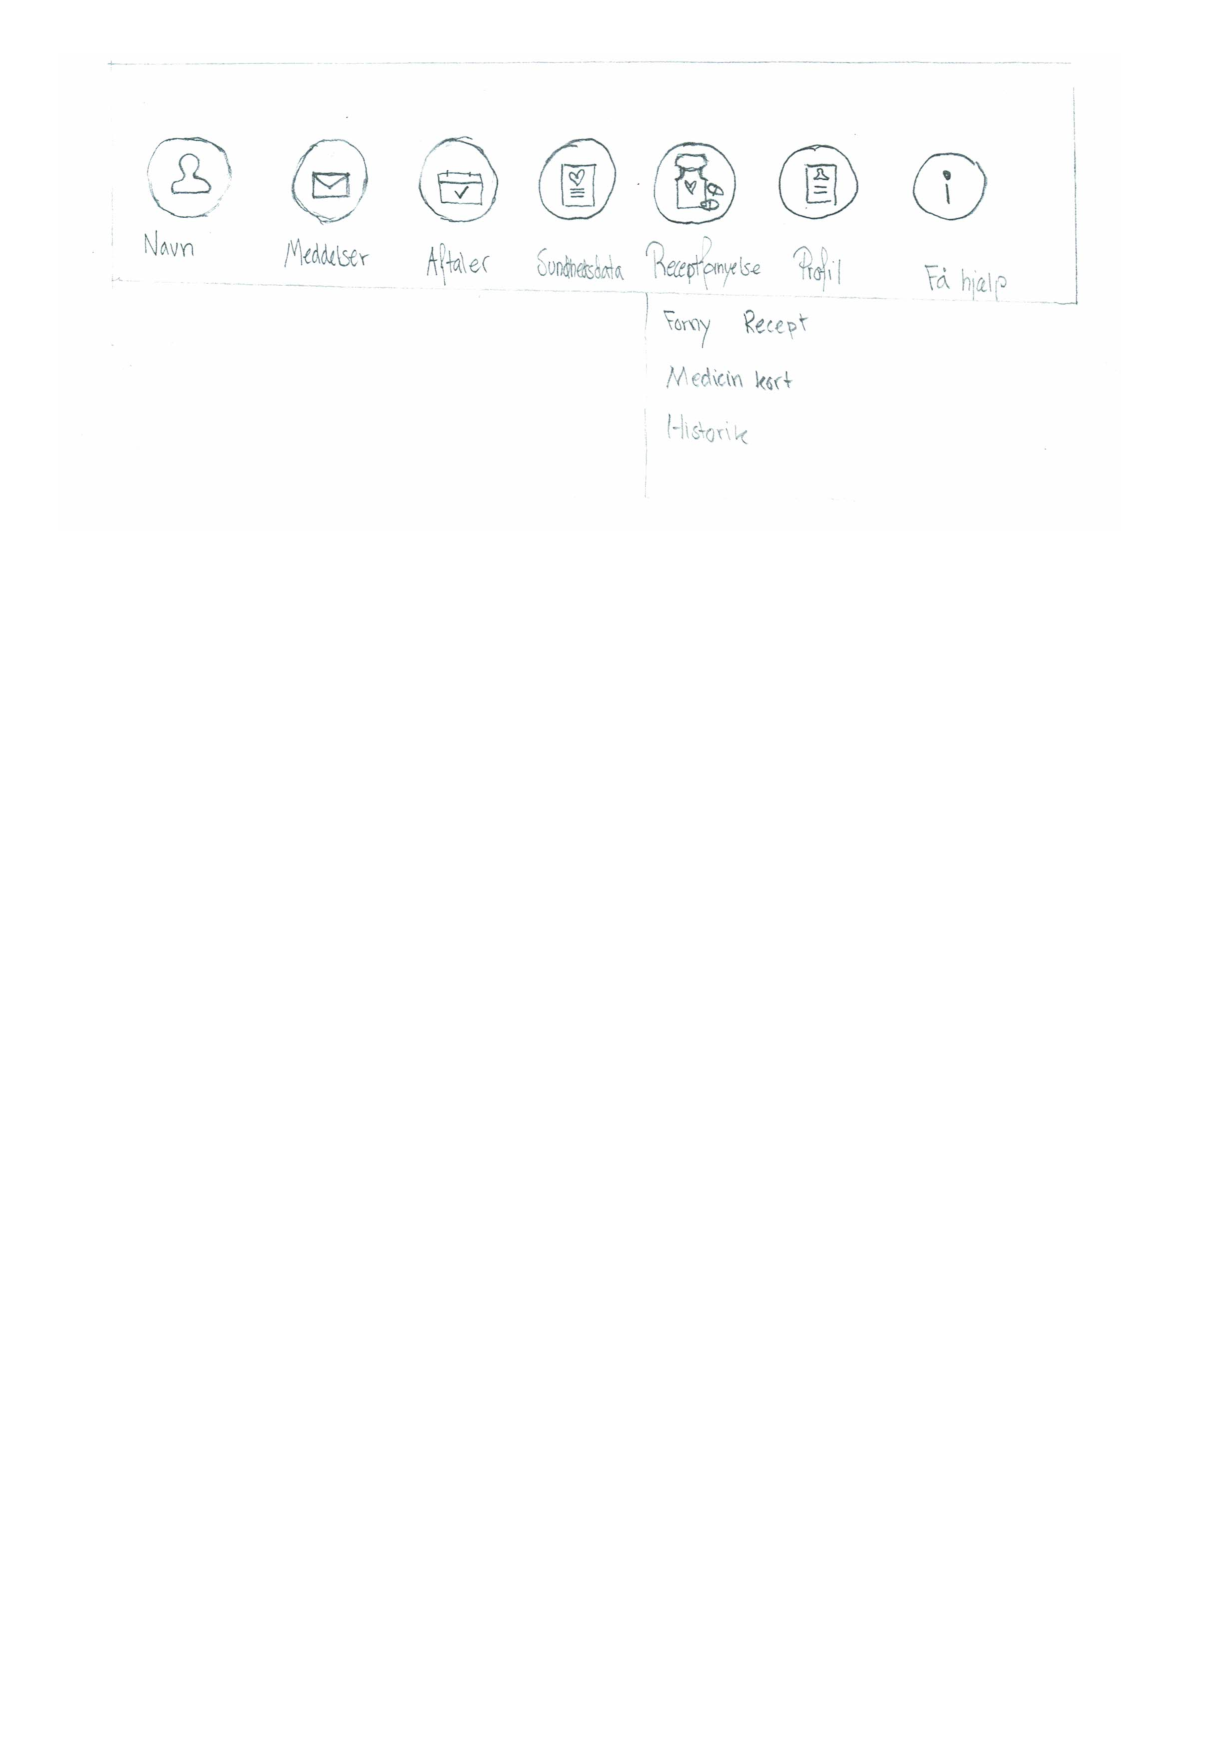
\includegraphics[angle=0, width=\linewidth]{Materials/FornyRecept_Hovedmenu.pdf}
	\caption{Mock-up for modulet 'Receptfornyelse': Hovedmenuen}
	\label{fig:Mock-Up1}
\end{figure}
Mock-up'en til Hovedmenuen med et 'Receptfornyelses-menu' er lavet med inspiration fra vores scenarier.\footnote{Bilag 5}
\begin{figure}[H]
	\centering
	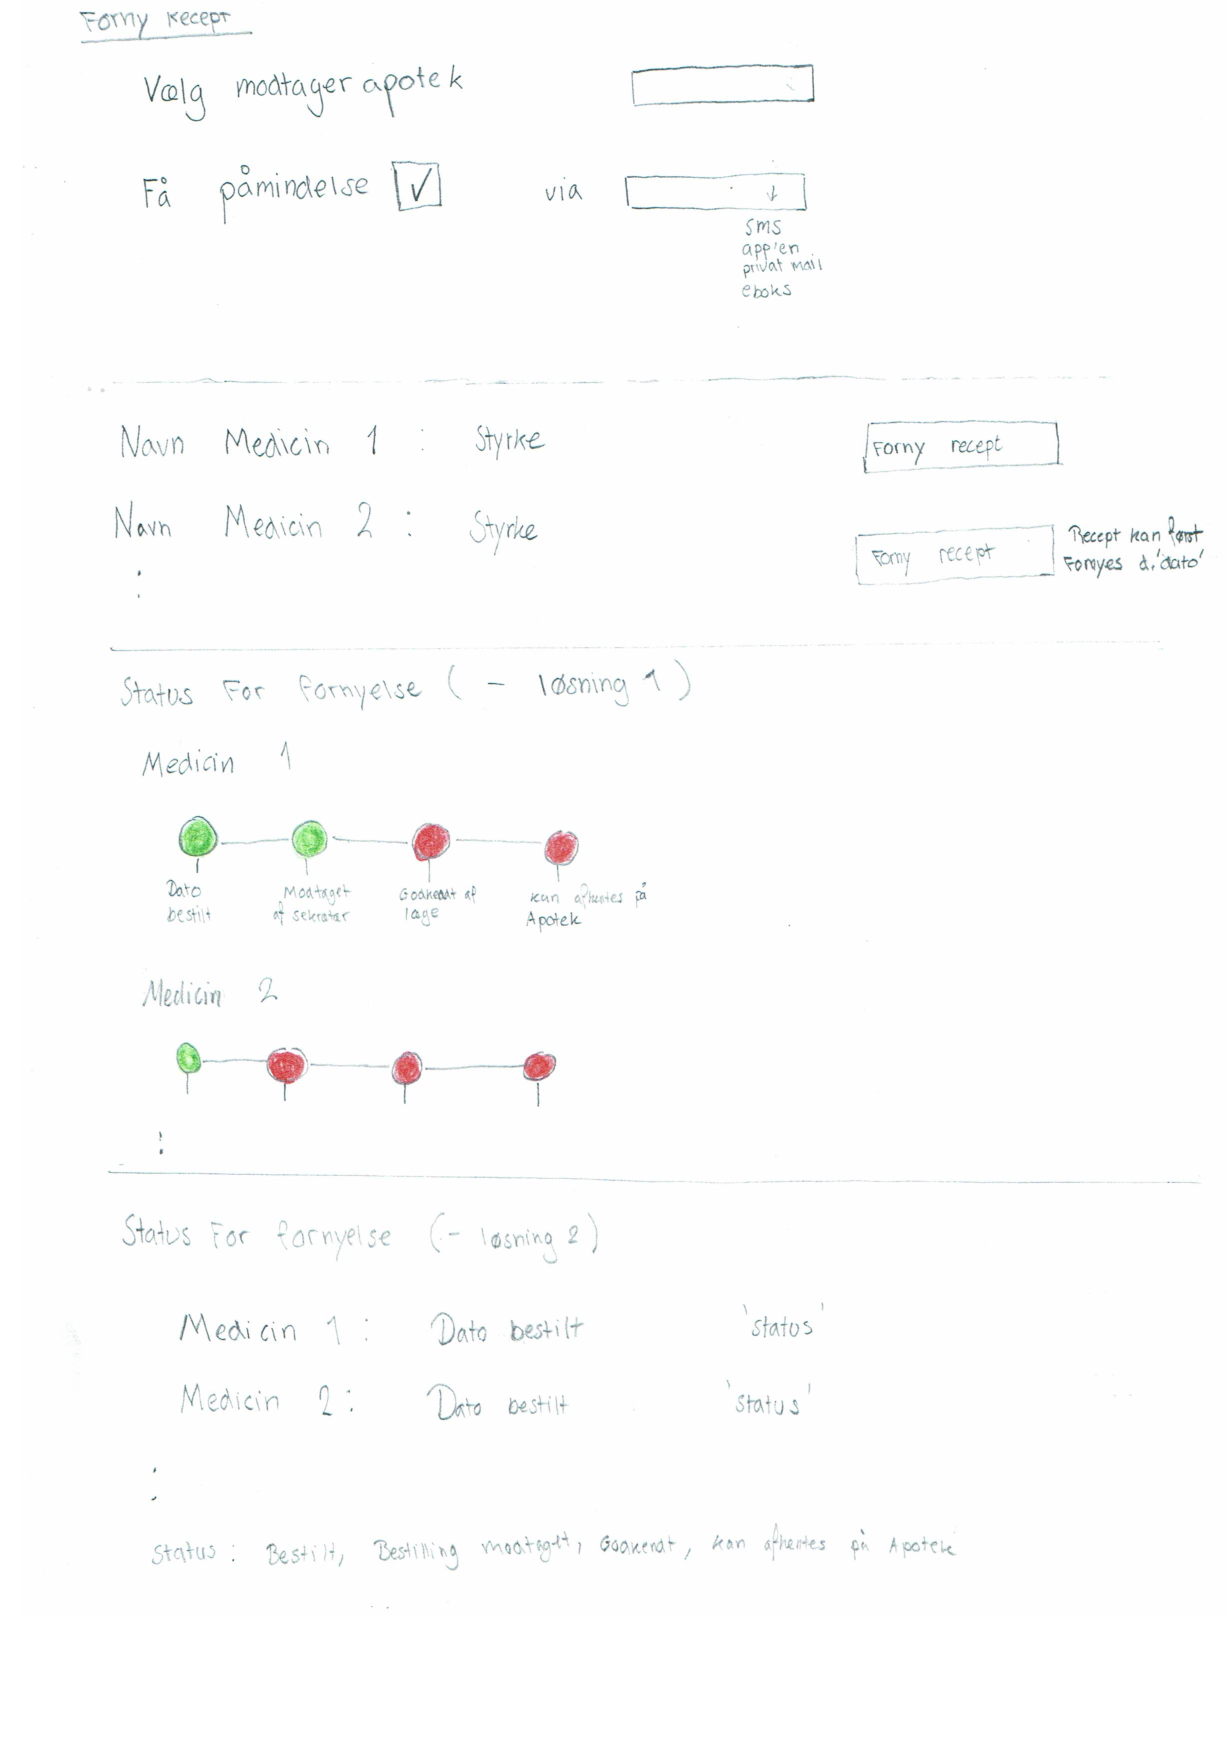
\includegraphics[angle=0, width=\linewidth]{Materials/FornyRecept.pdf}
	\caption{Mock-up for modulet 'Receptfornyelse': Undermenu, 'Forny recept'}
	\label{fig:Mock-Up2}
\end{figure}
I 'Vælg modtagerapotek' skal man i en drop-down menu kunne vælge mellem de to apoteker, som er tættest på en.\\
Hvis patienten ønsker påmindelse om receptfornyelse, skal patienten sætte hak ved 'Få påmindelse'.\\
Bemærk at knappen 'Forny recept' skal være blokeret i perioden, hvor recepten ikke må fornys. Der skal udover indformeres om, hvornår patienten igen kan forny sin recept, f.eks. med tekst ved siden af 'Forny recept'-knappen som vist i mock-upen.\\
Når patienten fornyer sin recept, skal der poppe en fortrydelsesbesked op, som siger: 'Er du sikker på du vil forny din recept?' hvor man skal kunne vælge 'Ja' eller 'Nej.\\
Der er to forslag til måden, hvorpå status for fornyelse kan vises. Statusmulighederne i løsning to er: Bestilt, bestilling modtaget, godkendt og kan afhentes på Apotek.\\
\begin{figure}[H]
	\centering
	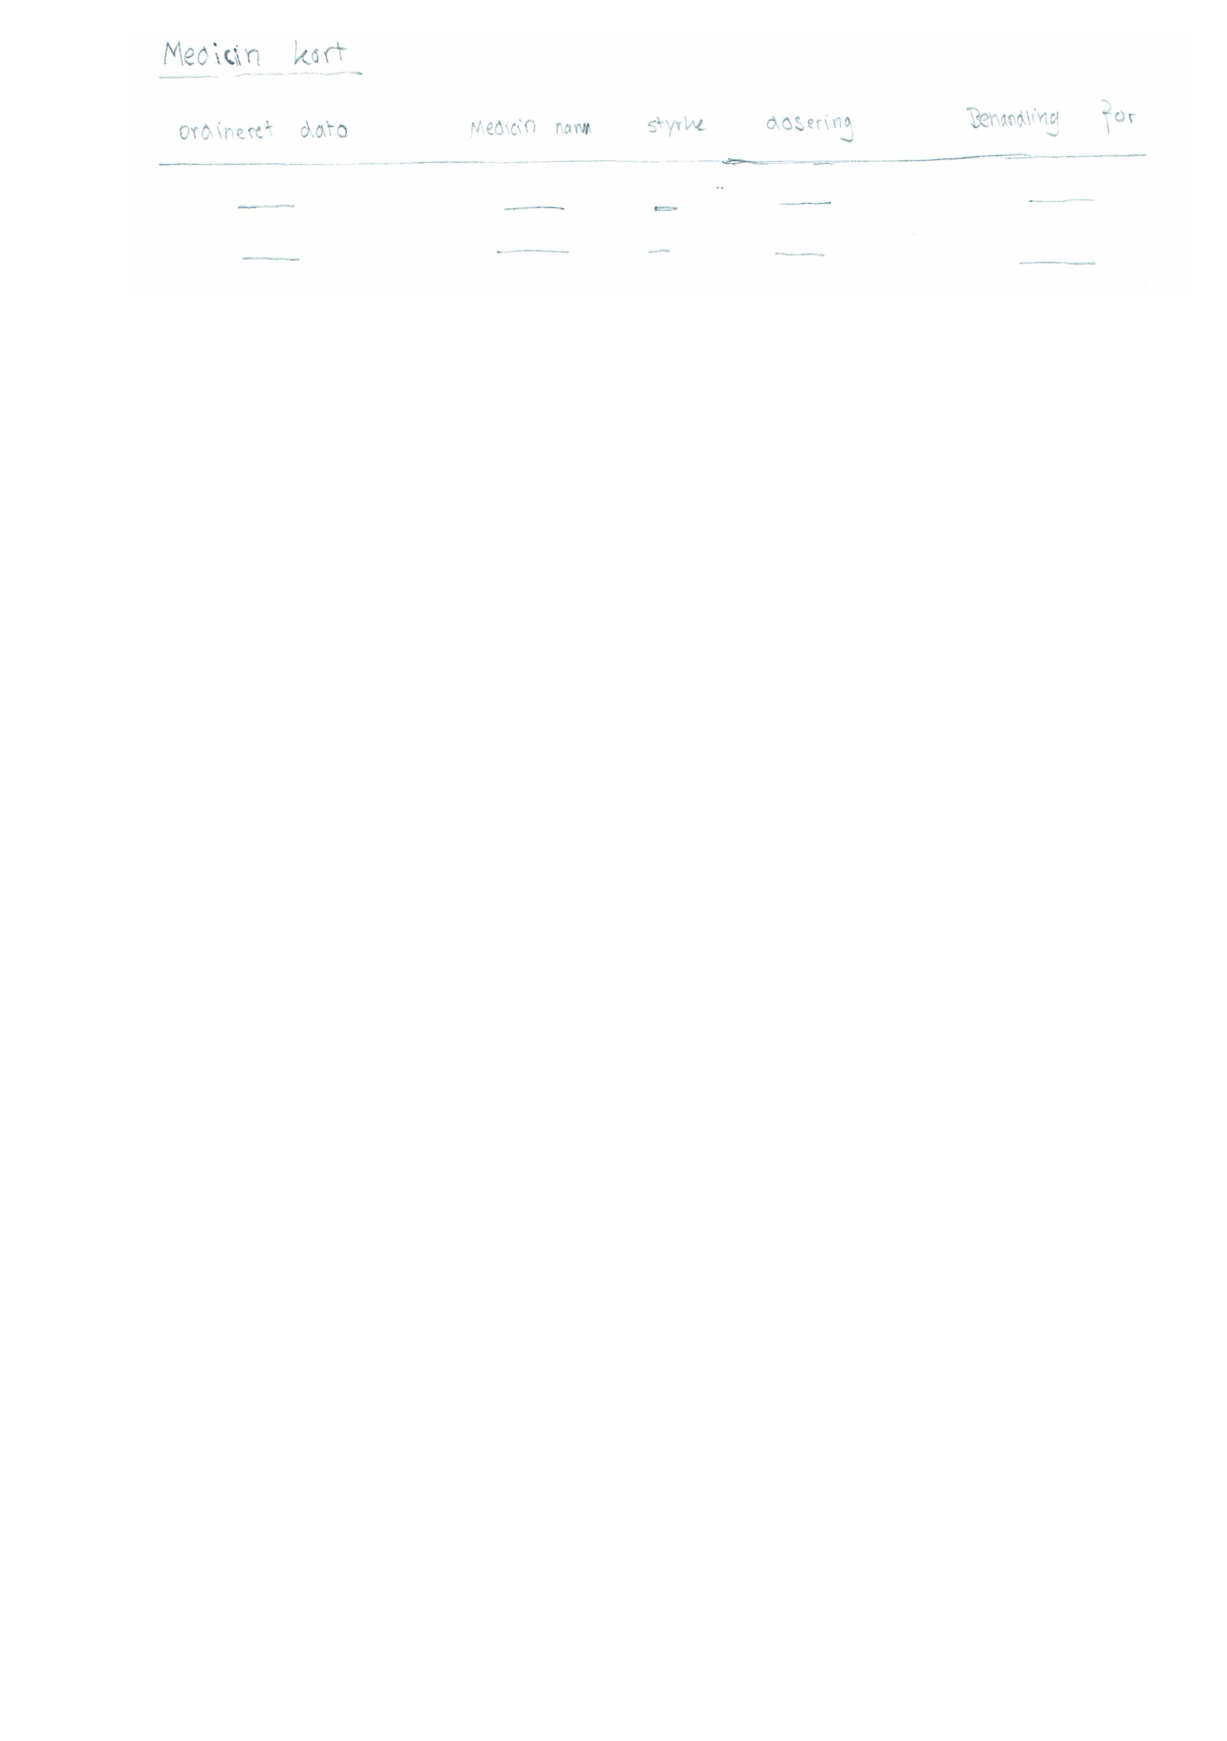
\includegraphics[angle=0, width=\linewidth]{Materials/FornyRecept_Medicinkort.pdf}
	\caption{Mock-up for modulet 'Receptfornyelse': Undermenu, 'Medicin kort'}
	\label{fig:Mock-Up3}
\end{figure}
\begin{figure}[H]
	\centering
	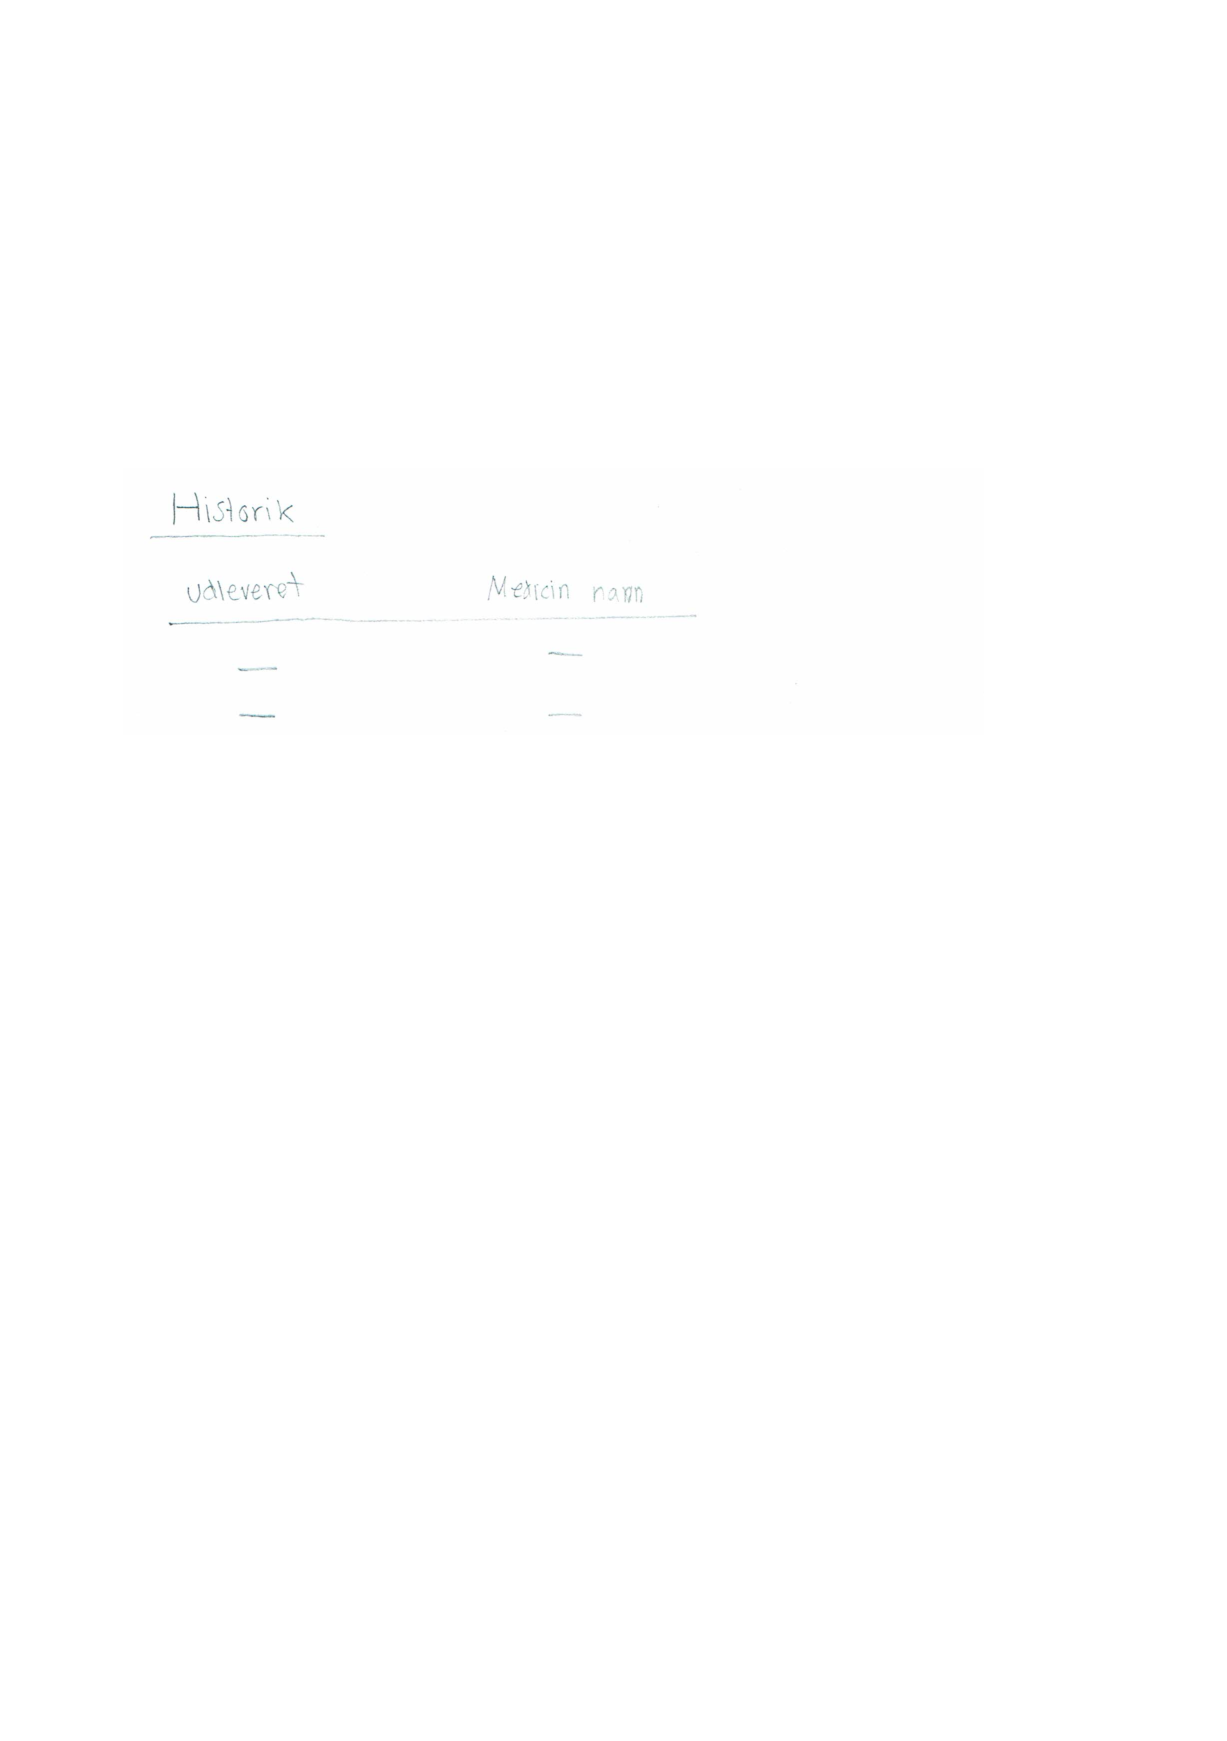
\includegraphics[angle=0, width=\linewidth]{Materials/FornyRecept_Historik.pdf}
	\caption{Mock-up for modulet 'Receptfornyelse': Undermenu, 'Historik'}
	\label{fig:Mock-Up4}
\end{figure}
% ? - Scenarios
\textbf{Samling af al information} \\
Forslag til brugergrænseflade for patienten fremgår af nedenstående Mock-up's:\\
\begin{figure}[H]
	\centering
	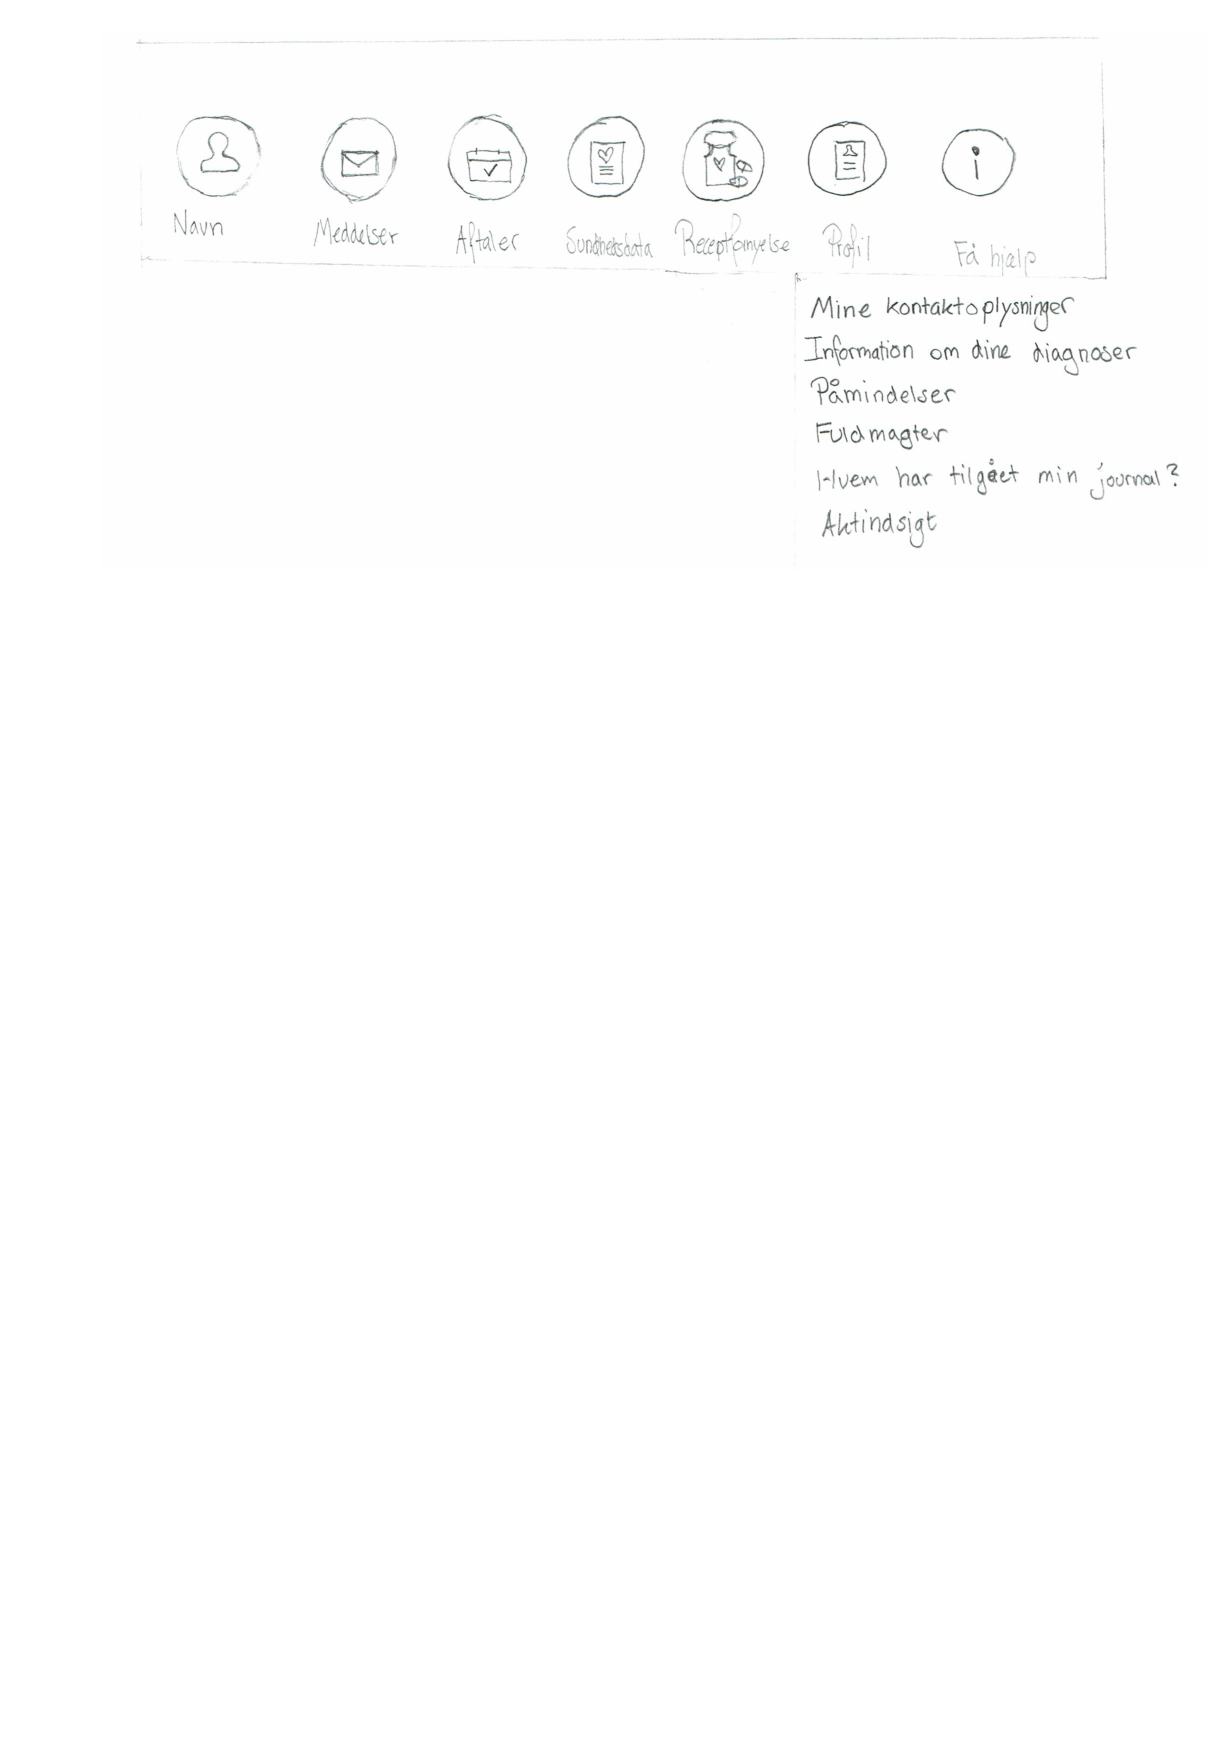
\includegraphics[angle=0, width=\linewidth]{Materials/Information_Hovedmenu.pdf}
	\caption{Mock-up for modulet 'Information om dine diagnoser': Hovedmenu, 'Profil'}
	\label{fig:Mock-Up5}
\end{figure}
Der er i hovedmenuen Profil tilføjet undermenuen 'Information om dine diagnoser'.
\begin{figure}[H]
	\centering
	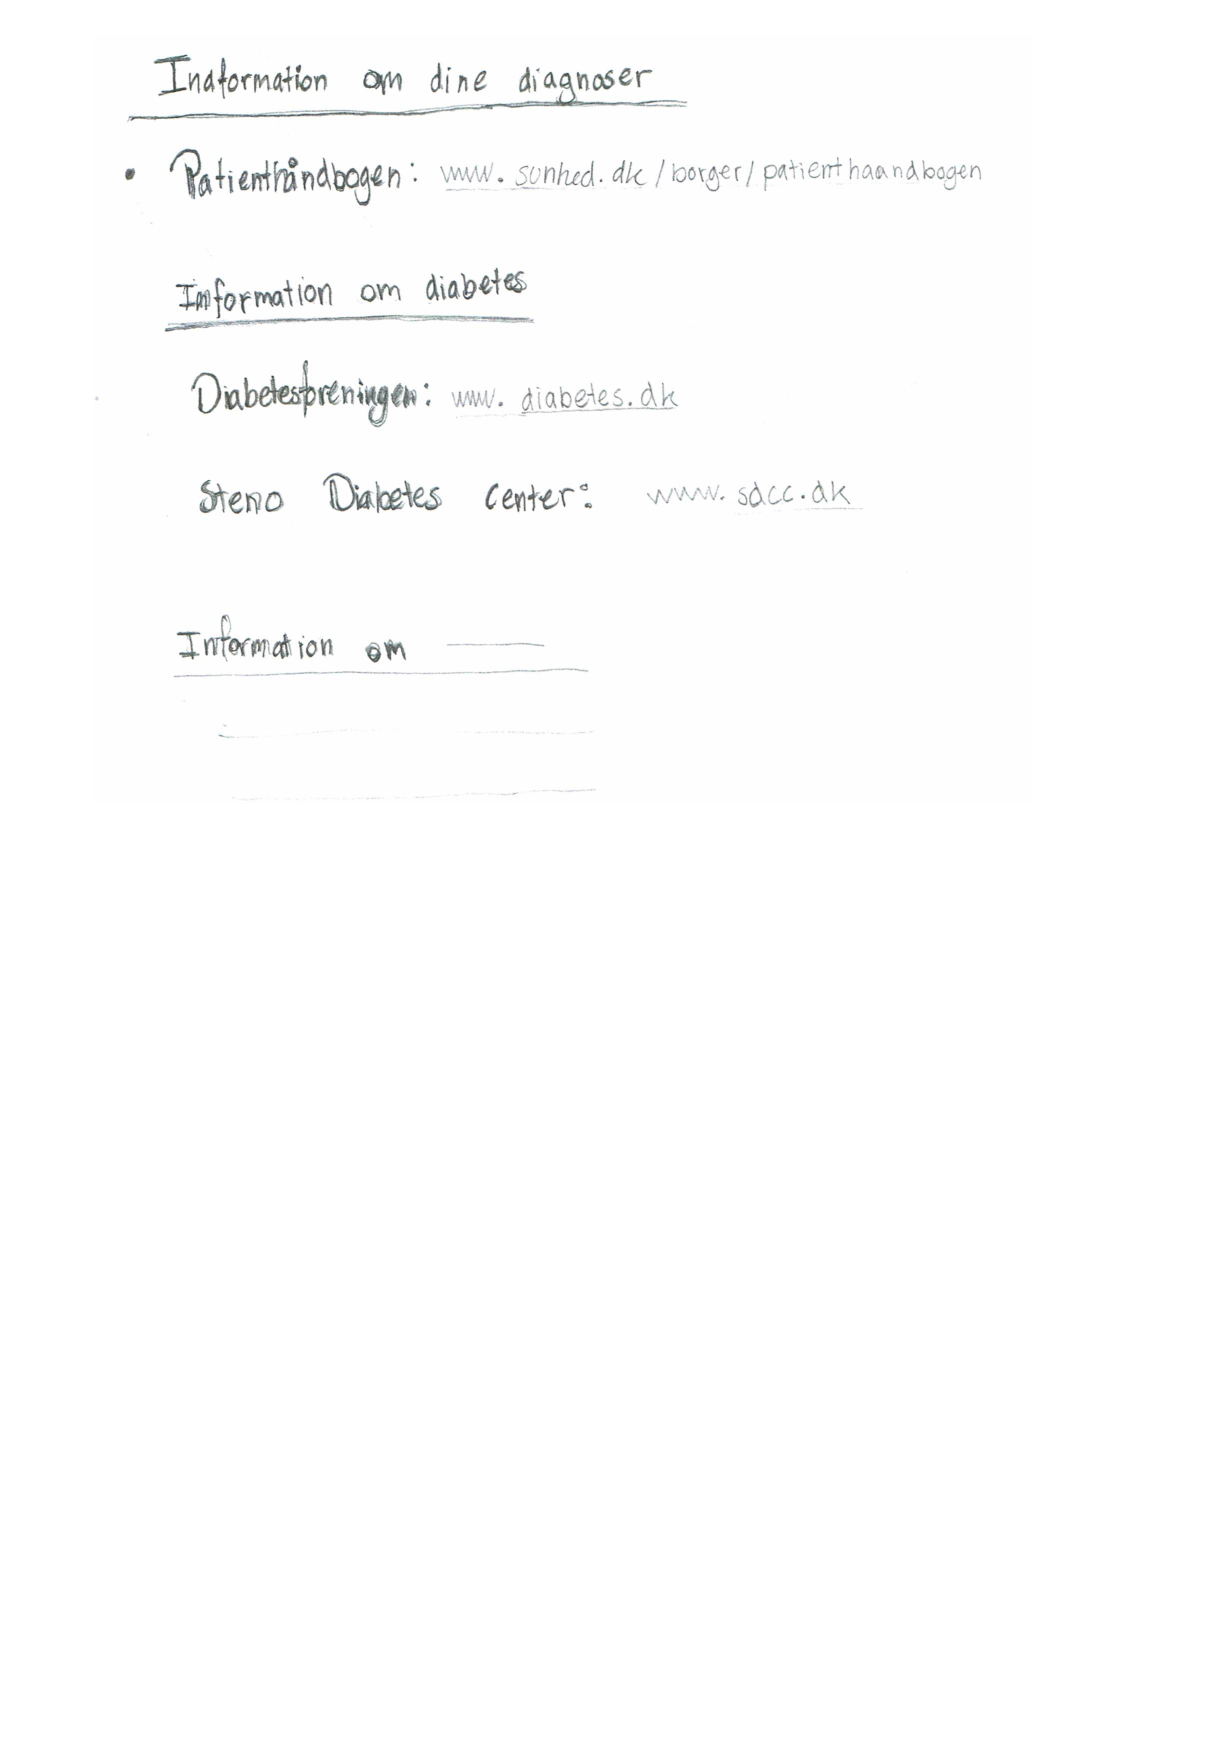
\includegraphics[angle=0, width=\linewidth]{Materials/Info2.pdf}
	\caption{Mock-up for modulet 'Information om dine diagnoser': Undermenu}
	\label{fig:Mock-Up6}
\end{figure}
Her kan patienten søge generel infomation om sin/sine diagnoser via links til relevante og anerkendte hjemmesider, der er udarbejdet af sundhedsfagligt personale.\\\\
\textbf{Uniforme Prøvesvar} \\
Forslag til brugergrænseflade for patienten fremgår af nedenstående Mock-up's:\\
\begin{figure}[H]
	\centering
	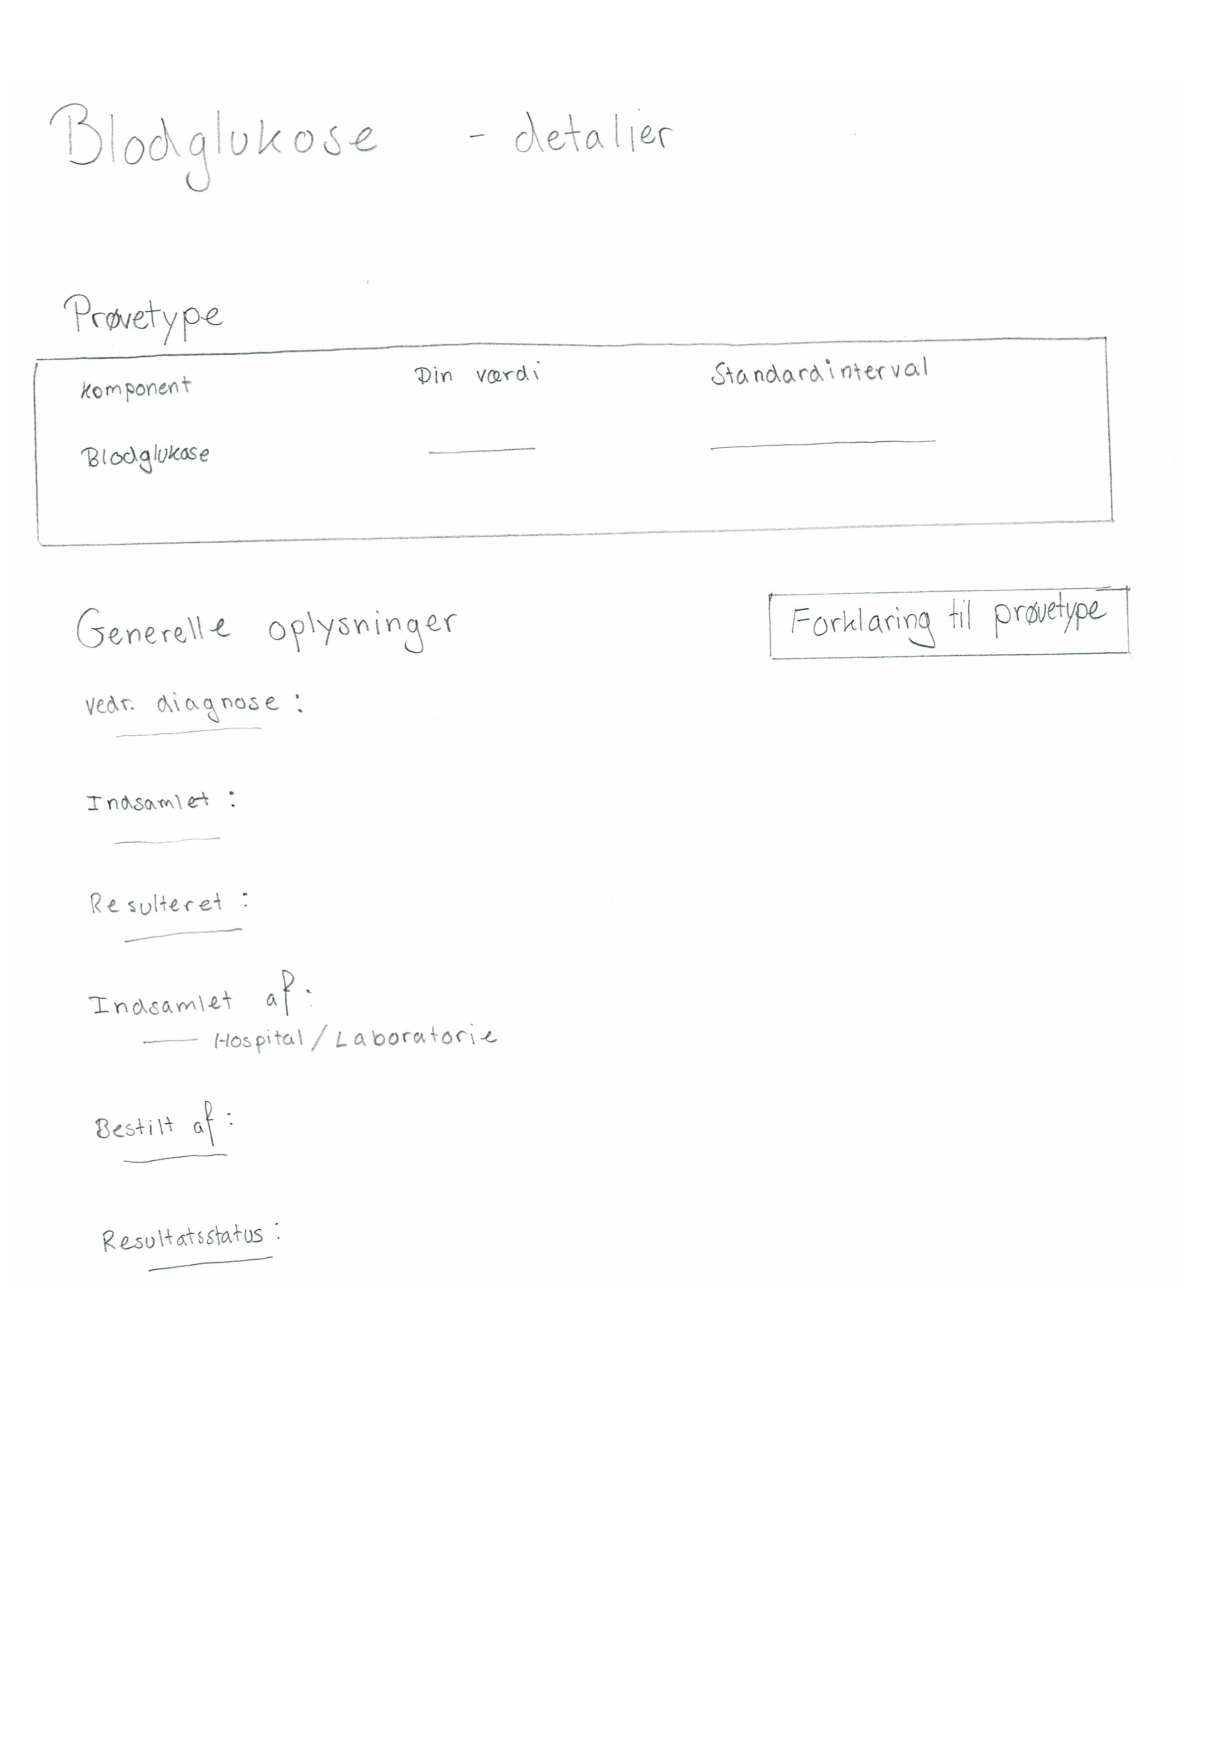
\includegraphics[angle=0, width=\linewidth]{Materials/provesvar.pdf}
	\caption{Mock-up for modulet 'Prøvesvar'}
	\label{fig:Mock-Up7}
\end{figure}
Når patienten klikker på knappen 'Forklaring til prøvetype' skal der vises en tekst på dansk med forklaringen til prøvetypen. Det kan laves som en pop-up eller ny side.\\

\subsection{Arbejdets organisering} 
Det lykkedes desværre ikke for os at få mulighed for at foretage virksomhedsbesøg. \footnote{Dybdeanalyse, afsnit 5 Konsekvensanalyse s. 18} Virksomhedsbesøg ville have givet os mulighed for at observere sundhedspersonalets nuværende arbejdspraksis, når patienterne fornyer deres recept via besked funktionen i MinSP og får taget prøver og givet prøvesvar.\\ 
Vi ville derfor bedre have kunnet vurdere hvilke ændringer, det giver i arbejdsorganisering for sundhedspersonalet og arbejdsfordelingen imellem læge, lægesekretærer, laboranter m.fl.\\
Vi havde også f.eks. haft mulighed for at observere forretningsgange, når patienterne bestilte receptfornyelse via sundhed.dk eller via en læges eget system, og fået inspiration til vores udvikling af receptfornyelse i MinSP.\\
Vi ville derfor have haft et bedre grundlag for at vurdere fordele og ulemper for sundhedspersonalet og relationerne imellem dem, deres arbejdsgange og evt. kvalifikationsbehov ved implementering af vores visioner.\\
Vi har derfor ikke haft den viden, som MUST-metodens princip om, at arbejdspraksis skal opleves ellers kunne have givet os. 
\\
\\
\textbf{Receptfornyelse} \\
En automatisk receptfornyelse vil muligvis ændre arbejdsgangen for sundhedspersonalet. \\ 
Lægen skal fortsat stadigvæk tjekke, at ordineringen er korrekt i forhold til journalen, men at læge-sekretæren slipper for at skrive besked tilbage til patienten, da patienten nu selv kan se forløbet i statuslinjen.
%
\\\\
\textbf{Samling af al information} \\
Hvis funktionaliteten implementeres via links som foreslået, vil der ikke være nogen ændringer til arbejdsgange og arbejdets organisering. \\
Hvis ikke funktionaliteten implementeres via links, men som en ny-udviklet informationside, er det sundhedspersonalet der skal skrive alt informationen/optage videoer mv., og siden vil skulle vedligeholdes af sundhedspersonalet, så det ville være en ekstra opgave, som sundhedspersonalet (læger, diætister og sygeplejeskær m.fl.) herved bliver pålagt.
\\\\
\textbf{Uniforme Prøvesvar} \\
Implementering af denne funktionalitet vil give ekstra arbejde for lægesekretæren eller laboratorie medarbejdere i forhold til indrapporteringen af prøvesvar, da der vil være flere informationer (navn på sted hvor prøven er taget og navn på diagnose), der skal indtastes, end med nuværende løsning. Der vil forinden være ekstra arbejde for lægen, da det er denne, der skal informere laboratorie-personale eller lægesekretær om, hvilken diagnose, de enkle prøvesvar vedrører.\\
Der skal tages stilling til hvor i organisationen indrapporteringen skal foretages. Desuden skal der nedsættes et udvalg enten på regionalt eller på landsplan som skal udarbejde standardsvarene til de uniforme prøvesvar.
\subsection{Kvalifikationsbehov}
\textbf{Receptfornyelse} \\
Receptfornyelses funktionaliteten vil ikke kræve nogen større oplæring af sundhedspersonalet, hvis de er rutinerede brugere af Sundhedsplatformen, men blot en introduktion til, hvordan den nye funktionalitet fungerer.
\\\\
\textbf{Samling af al information} \\
Hvis funktionaliteten implementeres via links, vil det ikke kræve nogen oplæring af sundhedspersonalet.
\\\\
\textbf{Uniforme Prøvesvar} \\
Vores vurdering er, at ændringerne ikke kræver ekstra kvalifikationer, da ændringen for sundhedspersonalet består i data-indtastning, som vi forudsætter at de allerede er bekendt med.
\\\\
Da vi ikke har haft mulighed for at foretage virksomhedsbesøg, har vi ikke haft kontakt med sundhedspersonalet i nogen af Region Sjællands hospitaler. Vi har derfor ikke haft mulighed for løbende at kunne informere personalet og ledelse om vores visioner til forbedring af MinSP som vi arbejdet med i dette forundersøgelses projekt. Vi har derfor ikke kunne opfylde MUST-metodens princip om forankring, hvor man fra forundersøgelsen første fase skal skabe forståelse og opbakning ved at informere alle interessenter der senere vil blive berørt af forandringerne. Det gælder både ledelse, sundhedspersonale og dem, der skal være ansvarlige for den tekniske og organisatoriske implementering.

        	\section{Vurdering af prioriteter og valg af prototype}
Efter en vurdering af vores prioriteter fra dybde analyse har vi som kandidater til forbedring af MinSP valgt følgende fokuspunkter: 'Receptfornyelse', 'Samlign af al information' og 'Uniforme prøvesvar'.
\\\\
Vores oprindelige prioritet 1 'Samling af al information' har vi nedprioriteret til prioritet 2. Vores argumentation herfor er, at det ville blive en for dyr løsning for sundhedspersonalet at vedligeholde. 
\todo{Casper: Hvad tænker du bliver for dyrt? 
	Svar: Jeg argumenterer for dette senere under Arbejdes organisering:
	Hvis en side skal ny udvikles og vedligeholdes, vil dette koste og derfor et det en dyr løsning. 
	Hvis siden skal ny udvikles er der nogen der skal skrive alt information / optage videoer osv. Derudover skal alt dette løbende holdes ajour af sundhedspersonalet. Det er derfor en dyr løsning.
	%
	% Note: skal der argumenteres mere her
} 
Ligeledes viste vores spørgeskemaundersøgelse, at 4 ud af 5 diabetiker, hvor den 5'te var neutral, ikke havde ønske om at MinSP skulle bruges til general information omkring sygdommen diabetes. Dette er dog i modstrid med vores interview-undersøgelse, hvor dette ønskes af de fleste.\\
For prioritet 2 'At skabe opmærksomhed omkring MinSP' og prioritet 3 'Overflod af fagtermer' har vi vurderet at løsningen ligger udenfor MinSP. Vores 3 prioritet bliver derfor 'Uniforme prøvesvar'.
\todo{Casper: Jeg forstår ikke sammenhængen?
	Svar: Vi har sagt at prioritet 2 og 3 ikke kan løses af os - ligger uden for min sundhedsplatformen. Derfor rykkes prioritet 4 op - for denne kan løses af os.
	%
	% Note: skal dette forklares på en anden måde
	% Note: Finn: Evt. brug Diagnostikkort, og senere Virtuellekort
}
\\\\
Det fremgår af Region Sjællands It-strategi \footnote{Projektgrundlag, s. 5, afsnit 3.1 IT Strategien}, at "...nye løsninger skal bruges i deres fulde omfang" og at patienterne og borgere skal opleve en bedre servicegrad og at de i så høj grad så muligt skal kunne betjene dem selv.\\
Som det fremgår af vores brugere-undersøgelser, fra både spørgeskemaer og interviews, er der ikke så mange der kender/bruger MinSP. Spørgeskemaerne viser, at 58,70\% ikke bruger MinSP, og på forespørgsel oplyser 84,6\%, at det er fordi, at de ikke kender MinSP. Dette fremgår også af vores interview undersøgelse, hvor 4 ud af 6 ikke kender MinSP.\\
Det er et problem for Region Sjælland, at patienterne ikke bruger MinSP, da det er en målsætning i Region Sjællands It-strategi \footnote{Projektgrundlag, s. 5-6, afsnit 3.1 IT Strategien}, at regionen ønsker fuldt udbytte af sine investeringer. 
Vi valgte derfor, at sætte 'At skabe opmærksomhed omkring MinSP', som anden prioritet i vores prioriteringsliste af fokuspunkter, men vurderet at dette problem lå udenfor MinSP. Det gjorder vi, fordi vi mener, at det er hospitalet selv og sundhedspersonalet, der har opgaven med systematisk at informere om MinSP. Dette kan ske ved f.eks. at udarbejde pjecer og fortælle om MinSP til diabetikerne via mails, eller når de kommer til kontrol på hospitalet. Der kan evt. også tilbydes læring i brugen af MinSP.\\
Imidlertid mener vi også, at en udvidelse af funktionaliteten, forbedring af brugervenligheden og af informationsniveauet, vil kunne understøtte en mere udbredt brug af MinSP.\\
Dette sammenholdt med, at vi ud fra vores spørgeskema undersøgelse kan se, at 57.1\% fornyer deres recept digitalt, gør, at vi har valgt at opprioriteret 'Receptfornyelse' (prioritet 8), til prioritet 1. Dette understøttes også af vores interview undersøgelse, hvor 4-5 ud af 6 diabetikere gerne vil forny deres recept digital, men bruger andre systemer som sundhed.dk eller deres læges eget system.
\\\\
Muligheden for at forny recept via MinSP kan kun ske som en skrevet besked til hospitalet, og funktionaliteten 'Receptfornyelse' er samtidig ikke særlig synlig, da den ligger under hovedmenuen 'Meddelelser' og undermenuen 'Skriv til os' og herefter først i en drop-down menu 'vælg emne' findes 'Receptfornyelse'. '\\
Vi mener derfor, at dette også er en årsag til, at patienterne ikke bruger dette modul, men bruger andre digitale sider. Ved at gøre tilgangen til modulet mere synligt, og samtidig videreudvikle det til en funktionalitet, hvor man hurtigere kan forny sine recepter samt have overblik over sin ordinerede medicin, mener vi, at det vil motivere patienterne til at bruge dette modul i MinSP. Dette også sammenholdt med, at vi udefra vores spørgeskemaundersøgelse kan se, at 21,43\% med sikkerhed, og 42,86\% sandsynligt ville forny deres recept via MinSP, mener vi, at disse ændringer ville kunne få flere til at bruge MinSP. Derved understøttes flere af målsætningerne i Region Sjællands It-startegi \footnote{Projektgrundlag s. 5-6, afsnit 3.1 IT strategien, punkt 2, 6 og 7}. Implementeringen af 'Receptfornyelse' understøtter også målsætningen i Region Sjællands it-infrastruktur om, at "Brugeren skal kunne finde løsninger i samme brugervendte arbejdsgange, uden at brugerne skal opleve behov for at navigere mellem forskellige løsninger"\footnote{Projektgrundlag s. 7, afsnit 3.4 It-infrastruktur, punkt 3}, da MinSP i højere grad bliver en samlet side for alle funktioner. 
\\ \\
Overnævnte argumentation er årsag til, at vi har opprioriteret prioritet 8 om 'Receptfornyelse' til prioritet 1. 
\\\\
Vi har derfor valgt 'Receptfornyelse' som den vigtigste forbedring og valgt at udarbejde en protype for denne funktionalitet.
        	% Konsekekvens-analyse resultatet giver Fordele og Ulemper
% ud fra Scenarios
%s. 207 Konsekvansanalyse: 'gennemgå systematisk de forslåene visioner'
%
%  Teknik: Virtuelle kort, evt. Brug SWOT s. 269-270, Design skitsere
%
% Pricippet Samlet Vision - s. 72 trekant:  IT-udvikling / kvalifikationsudvkling / Organisatoriske udvikling : 
%
%Diskution af
% hvad er ændringen
% hvordan pårvirker det mennesker der skal bruge det
% Arbejds Organiserings ændringer / skaber det ændringer i arbejdsgange
% Forankring ('knytter sig til' personalet og organiserings)
% krav til uddanelse /kvalifikations krav
% Økonomi
% /Matcher det med Region H. forretnings og IT stategi
\section{Konsekvensanalyse: Fordele og Ulemper}
I dette afsnit ser vi på hvorfor visionerne er relevante for Region Sjællands forretnings- og it-strategi, for sundhedspersonalet og for patienter og lervandører. \\
Til hjælp i vores vurdering af fordele og ulemper af visionerne om 'Receptfornyelse' og 'Samling af al information' på MinSP, har vi udarbejdet to scenarier, hvor visionerne ses ud fra henholdsvis en bruger og en sundhedsfagligs synspunkt. Scenarierne ses nedenfor under \textcolor{red}{punkt 6}.
\todo{Virtuelle kort / SWOT analyse}
\subsection{Region Sjællands forretnings- og it-strategi}
\textbf{Prioritet 1, Receptfornyelse}\\
Fordelen ved at implementere en automatisk receptfornyelses funktionalitet er, at brugerne kan betjene sig selv og vil opleve en bedre service. Det vil muligvis også reducere sundhedspersonalets ressourceforbrug. Dette opfylder målsætninger i Region Sjællands it-strategi \footnote{Projektgrundlag, s. 6, Afsnit 3.1 IT strategien, punkt 7 }.\\
Det vil også opfylde Region Sjællands it-strategi om infrastruktur, at MinSP bliver en samlet side for alle funktioner og har integrerede selvbetjenings løsninger. \footnote{Projektgrundlag, s. 7, Afsnit 3.4 It-infrastruktur punkt 3 og 4}\\
Ulempen er, hvis funktionaliteten 'Receptfornyelse' ikke bliver brugt af patienterne, men at patienterne i stedet stadigvæk bruger sundhed.dk, fordi vi vuderer, at funktionaliteten vil være rimelig dyr at implementere, og det vil være i modstrid med Region Sjællands it-strategi om at "Regionen vil have fuldt udbytte af sine investeringer, og de nye løsninger skal bruges i deres fulde omfang" \footnote{Projektgrundlag, s. 5, Afsnit 3.1 IT strategien, punkt 2}. Det vil sige, at det så vil være en dårlig cost/benefit for regionen.\\ 
En bedre løsning ville så være kun at oprette den nye hovedmenu 'Receptfornyelse' og herunder linket til sundhed.dk. Det vil dog være i modstrid med Region Sjællands it-infrastruktur, om at "Brugeren skal kunne finde løsninger i samme brugervendte arbejdsgange, uden at brugerne skal opleve behov for at navigere mellem forskellige løsninger" \footnote{Projektgrundlag, s. 7, Afsnit 3.4, It-infrastruktur, punkt 3}. 
\\\\
\textbf{Prioritet 2, Samling af al information}\\
En 'standardløsning' med link til sider med information om diabetes stemmer overens med Region Sjællands forretnings- og it-strategi om, at patienter i så høj grad som muligt skal kunne betjene sig selv samtidig med, at de får en bedre servicegrad og regionen reducerer sit ressourceforbrug. \footnote{Projektgrundlag, s. 6, Afsnit 3.1 IT strategien, punkt 7} \\
Det er også en prioritet i it-strategien, at systemer skal kunne hente information fra andre systemer, så dette understøttes også af vores løsning. \footnote{Projektgrundlag, s. 6, Afsnit 3.1 IT strategien, punkt 8} \\
Løsningen opfylder også en målsætning i regionens it-infrastruktur om at: "Regionen ønsker systemer, som kan hente information fra andre systemer, således at brugeren kun skal henvende sig et enkelt sted".\footnote{Projektgrundlag, s. 7, Afsnit 3.4 It-infrastruktur, punkt 3}
\\\\
\textbf{Prioritet 3, Uniforme Prøvesvar}\\ % ? - Er løsningen dyr at kode
En forbedret løsning til visning af prøvesvar vil give patienterne bedre service som er i overensstemmelse med regions it-strategi. \footnote{Projektgrundlag, s. 6, Afsnit 3.1 IT strategien, punkt 7}\\
Det er det sundhedsfaglige personale, der skal lave de danske beskrivelser for de forskellige typer af prøvesvar. Dette matcher ikke med Region Sjællands ønske om at reducere sit ressourceforbrug \footnote{Projektgrundlag, s. 6, Afsnit 3.1 IT strategien, punkt 7}, så cost/benefit skal vurderes i forhold til det forbedret service niveau for patienterne. 
\subsection{Relationer mellem sundhedspersonalet og mellem afdelinger}
\textbf{Prioritet 1, Receptfornyelse}\\
Det er en fordel for læge-sekretærerne, at de ikke længere skal huske at svare tilbage til patienter omkring receptfornyelse og skal bruge tid på det.
% Ulemper -?
\\\\
\textbf{Prioritet 2, Samling af al information}\\
Det er en fordel for sundhedspersonalet, at patienterne i højere grad selv kan søge information, da det vil betyder mindre arbejde for sundhedspersonalet.\\
Det vil give en bedre kommunikation mellem sundhedspersonalet og patienterne, når patienter, via informationslinksene, er bedre informeret om deres sygdom, behandlingsforløb, kost og motion m.v.
% Ulemper -?
\\\\
\textbf{Prioritet 3, Uniforme Prøvesvar}\\
Prøvesvarene bliver mere forståelige for patienterne, og det vil lette arbejdet for sundhedspersonalet med at besvare spørgsmål og forklare prøvesvar for patienterne.\\
Det er en ulempe, at sundhedspersonalet får mere arbejde med at indrapportere ekstra data. \\ Det er også sundhedspersonalet, der skal lave de danske tekster.
\subsection{Patienter og lervandørere}
\textbf{Prioritet 1, Receptfornyelse}\\
Patienter kan bestille receptfornyelse det samme sted, som hvor de kan se prøvesvar og kommunikere med hospitalet, og de kan følge med i, hvor langt deres bestilling er nået.\\
Det kommer muligvis til at gå hurtigere for patienten at få fornyet sin recept, fordi der ikke skal skrives beskeder til hospitalet. Patienten undgår arbejdet med at skrive beskeder og at skulle huske, hvad medicinen hedder.\\
Patienten får også et medicin kort, der er nemt at finde og adgang til en historik over, hvad de har fået af medicin gennem tiden i deres sygdoms forløb.\\
Der tages hensyn til brugervenligheden ved at gøre receptfornyelses modulet synligt.\\ 
Der er ingen ulemper for patienten, for de vil stadigvæk kunne bruge sundhed.dk eller kunne kontakte egen læge, hvis de hellere vil det.\\
Apoteket vil muligvis komme til at skulle tjekke to steder for medicin bestilling: sunhed.dk og MinSP.
\\\\
\textbf{Prioritet 2, Samling af al information}\\
Ifølge vores interview-undersøgelse har det at kunne søge information og vejledning om sin sygdom været meget efterspurgt. Så løsningen vil opfylde et stort behov hos brugerne. \\
Linket til patienthåndbogen er gjort mere synlig ved at være flyttet fra "Historik" under "Sundhedsdata" til "Information om dine diagnoser" under "Profil". Det har gjort informationssøgning på MinSP mere brugervenlig for patienterne.\\
Vi har udvidet med to ekstra informationslink, hvor patienterne kan finde information om nogen af de forhold de har efterspurgt, f.eks. video om hvordan man måler blodglukose, kost-vejledning mm.\\
Det er nemt at udvide modulet med flere informationssider, hvis dette ønskes af patienterne.\\
Der skal muligvis skaffes tilladelse fra leverandørerne af linksene til at bruge linksene.
% Patienter og levandørere: de skal sige god for til links i 'Samling af al information'
\\\\
\textbf{Prioritet 3, Uniforme Prøvesvar}\\
Patienterne vil bedre kunne forstå, hvad et prøvesvar omhandler, når der er tilknyttet en standard beskrivelse på dansk. Patienten vil også kunne se, hvor deres prøver er taget.\\ Begge tilføjelser er, jf. vores interviews, et ønske fra patienterne.\\
Ved at samle prøvesvarene pr. diagnose giver det patienterne et bedre overblik over deres prøvesvar.
        %	\section{Baggrund og fokus}
Nedenfor ses et sammendrag af vores interviews med vores deltagende diabetes patienter.
\subsection{Interview - Jannie}
Jannie er på førtidspension og har tidligere været pædagog i 8 år. Jannie er normal af bygning, spist almindelig sund kost og altid været sund og rask. Af disse årsager vælger hun i år 2002 at tage forbi Amager Hospital, hvor hun gerne vil melde sig som bloddoner. Dette skal vise sig at være hendes første møde med diabetes på nært hold. Blodprøven viste et højt blodsukkertal og ved senere lægetjek fik hun konstateret diabetes type-2.
\\ \\
I dag tager Jannie medformin 2 gange om dagen og stikker sig med ”insulin-booster” én gang om ugen, hvilket hun beskriver som værende her, at hun for alvor føler at hun er syg. At stikke sig har altid været ubehageligt og sygdomspåmindende i forhold til medformin, som er på tablet-form. Jannie lever som førtidspensionist et meget aktivt liv, hvor hun i ugens løb går til; Yoga mandag, Ipad-kursus tirsdag, synger i gospelkor onsdag, og er frivillig ved hus forbi om torsdagen.
\\ \\
Jannie beskriver sig selv som værende teknisk rutineret, men deltager som førnævnt til Ipad-kursus og vil hele tiden gerne blive klogere på den digitale-verden. Heraf blev dette interview også afholdt via facetime som hun for nyligt var blevet undervist i. Af digitale platforme med relevans for diabetes har Jannie blandt andet benyttet facebook, men har kort inden interviewet afmeldt sig diverse diabetesgrupper, da den løselige information på dette medie ikke sagde hende noget. Herudover benytter hun ”nettet” til informationssøgning – intet specifikt. Jannie har desuden en datter, der læser en sundhedsrelevant uddannelse og får derigennem en masse information vedrørende kost og motion.
\\ \\
Jannie kender ikke til minsp.dk, men er tilknyttet diabetesafdelingen på Amager Hospital, hvor hun kommer ca. hver 3. måned. Her bliver hun vejet, målt, får taget blodprøver og en gang i mellem deltager i lægekonsultation. Hun går desuden også hos egen læge og bestiller tid og recept til hendes medicin igennem lægens eget interne system.
Som afsluttende del af interviewet spurgte vi Jannie om, hvorvidt hun havde en skør idé til en fremtidig digital platform, som kunne hjælpe diabetikere. Et forslag til en ren digital løsning havde hun ikke, men havde som diabetiker ønsket, at hendes sygdomsforløb havde været grebet anderledes an i starten. Hun ville ønske, at der i fremtiden blev sat mere fokus på behandling for nyligt diagnosticerede diabetikere således, at de hurtigt og effektivt kunne blive sat i gang med deres behandling, og at informationsniveauet både var højere og mindre medicinsk anlagt. Hun foreslår, at en personlig vejleder kunne være en mulig løsning (f.eks. en sygeplejeske), der i starten kunne hjælpe én på rette vej – dette kunne evt. sagtens ske via en platform som minsp.dk og via webcam, foreslår hun.

\subsubsection*{Think aloud – minsp.dk}
Jannie logger på minsp.dk på sin Ipad og skal først tilmelde sin e-mail, da det er første gang hun logger på. Herefter tilgår hun de forkellige funktioner på siden. Hun har aldrig været på siden før og  læser op imens hun navigerer rundt: ”Se din 14 seneste tests” siger hun, og trykker sig ind. Hun bliver henrykt over at kunne se sine resulater fra Amager Hospital og oplæser en masse latinske lægefaglige udtryk, som hun ikke forstår og siger ”Hvordan skal jeg på nogen måde kunne forstå disse ting”. Hun navigerer videre på siden og finder hendes andre diagnoser: diabetes type-2, rygsmerter og diskoskolaps. "Ja det passer jo, det har jeg også", siger hun så. Resten af navigationen rundt på siden sker uden problemer, og hun synes, at den virker intuitiv og ret brugervenlig. 

\documentclass[english]{article}
\usepackage[utf8]{inputenc}
\usepackage[T1]{fontenc}
\usepackage{babel}
\usepackage{amsmath}
\usepackage{graphicx}
\usepackage{fancyhdr}
\usepackage{listings}
\usepackage{textcomp}
\usepackage{siunitx}
\usepackage{xcolor}
\usepackage{listings}
\definecolor{commentgreen}{RGB}{2,112,10}
\definecolor{eminence}{RGB}{108,48,130}
\definecolor{weborange}{RGB}{255,165,0}
\definecolor{frenchplum}{RGB}{129,20,83}
\lstset {
    language=python,
    frame=tb,
    tabsize=4,
    showstringspaces=false,
    numbers=left,
    upquote=true,
    commentstyle=\color{commentgreen},
    keywordstyle=\color{eminence},
    stringstyle=\color{red},
    basicstyle=\small\ttfamily, % basic font setting
    emph={int,char,double,float,unsigned,void,bool},
    emphstyle={\color{blue}},
    escapechar=\&,
    % keyword highlighting
    classoffset=1, % starting new class
    morekeywords={>,<,.,;,,,-,!,=,~},
    keywordstyle=\color{weborange},
    classoffset=0,
}
\pagestyle{fancy}
\fancyhf{}
\renewcommand{\headrulewidth}{0pt}
\setlength{\headheight}{0pt} 

\begin{document}

\section*{Interview - Ernst}
Ernst er type-2 diabetiker og arbejder til dagligt som buschauffør. Ernst fik konstateret diabetes tilbage i år 2005, hvor han som bloddoner fik en melding om alt for højt blodtryk. Derfor kom han  til kontrol hos egen læge, hvor han herefter fik sin diagnose.
I starten gik han til egen læge hver 3. måned og fik medformin, som er tablet-medicin for diabetikere. I starten tog Ernst meget let på sin sygdom og de første mange år gik han uden at ændre sin livsstil. Ernst led af stor overvægt og dårlige madvaner – heraf fortalte Ernst at han især var glad for ostemader, hvor 10 stk. dagligt ikke var helt ualmindeligt.
Omkring år 2015 får Ernst beskeden om at han skal være bedstefar, dette var en stor øjenåbner for ham og et opråb om at en livsstilsændring skulle til for at hans levealder og tid sammen med barnetbarnet kunne forlænges. Hans startede derfor hvor det stod værst til – ved hans livstil.
\\ \\
Ernst vælger at tilmelde sig TV2 programmet “Kan man spise sig rask”, hvor han bliver castet, deltager og opnår flotte resultater. Siden har han taget en Umahro-uddannelse (Sundhedsrådgiver) og hjælper ligesindede ved at brede sit budskab vedr. diabetes, og hvordan man kan behandle sin sygdom på andre områder end via de medicinske veje, som han oplever har været omdrejningspunktet i de lægefaglige kræse – hvilket han har en meget stærk holdning til. Herudover er Ernst tilknyttet frivilligcenteret i kommunen, hvor han fortæller og vejleder i KRAM-faktorene (Kost, rygning, alkohol og motion)
\\ \\
Ernst kender ikke til minsundhedsplatform.dk, men er dog tilknyttet Nykøbing Falster Sygehus, hvor han deltager i årlig kontrol. Muligheden for mindst én kontrol årligt som diabetiker blev han først opmærksom på efter, at have været hos egen læge i flere år og har tidligere haft dårlige erfaringer med sin egen læge og dertilhørende henvisninger til informative og støttende foreninger for diabetikere. Det var først da Ernst, fik sit barnebarn at han vendte op og ned på sit liv. 
\\ \\
Ernst er som tidligere nævnt tilknyttet Sygehuset i Nykøbing på Lolland Falster, hvor han årligt går til kontrol. Han mener at fagpersonalet har valgt at sende ham e-mails med de prøvesvar og kontroller han har gået til, men har tilsyndeladende ikke tjekket op på dette et stykke tid, da han ikke rigtigt kan huske det. Han mener at han stadigvæk får e-mails tilsendt, og har hvertfald ikke været opmærksom på minsp.dk. Ernst foretrækker personlig kontakt, hvorfor han i dag også fornyer sin recept via telefon og ikke via lægens interne systemer. Af andre digitale platforme benytter Ernst facebook, hvor han fortæller og rådgiver andre diabetikere med sine egne erfaringer, men er samtidig også skeptik og afholdende fra at modtage gode råd fra disse grupper.
\\ \\
Generelt er Ernst utilfreds med den måde, hvorpå hospitalsvæsenet håndterer diabetes idet, at han får for lidt information omkring alternativ sygdomsbekæmpelse end den medicinske. Han mener at det er økonomiske årsager mellem det offentlige og medicinindustrien der spiller en væsentlig rolle for denne behandlingsmetode. Han fortæller at han var underinformeret omkring blandt andet aflæsning af tal og hvordan han skulle gribe sin livsstilsændring an igennem mange år af sit sygdomsforløb. Ernst savnede især “gode eksempler” hvilket han foreslå for eksempel kunne komme via video på nettet. Overordnet har Ernst manglet motivation og information omkring hvor og hvordan han kunne blive klogere på metoder til at takle sin dagligdag fra den dag han fik konstateret diabetes.

\subsection*{Think aloud – minsp.dk} 
Ernst loggede på minsp.dk via hans computer og fandt platformen ret intuitivt. Her kunne Ernst tilgå de forskellige funktioner på siden uden problemer og viste stor interesse og nysgerrighed om denne side han ikke før havde hørt om. Han kiggede på nogle tidligere journaler, men var dog i tvivl om nogle af de aktuelle journalers indhold, om hvorfra og hvilken kontrol disse stammede fra. Han havde ikke yderligere kommentarer til siden som helhed og indtrykket var overordnet positivt.



\end{document}
\subsection{Interview - Karen}
Karen er pensioneret sekretær og fik konstateret type-2 diabetes i en ret ung alder. I starten fortalte hun at hun var meget underinformeret, hvor hun var bange for sin sygdoms konsekvenser og ikke vidste hvordan hun skulle håndtere sin sygdom. Dette fik hende til at spise utrolige mængder rugbrød uden pålæg som et desperat forsøg på at komme hendes sygdom til livs, hvilket resulterede i at hun tog meget på i vægt i den periode. Hun mente at informationsniveauet i starten var utilstrækkelig og manglede generelt information til hvordan hun skulle gribe sin sygdom an i forhold til fremtidig bahandling. I dag tager hun medformin, 2 piller morgen og aften, og lever et godt og aktivt liv trods sin sygdom.
\\ \\
Karen har tidligere været tilknyttet Bispebjerg sygehus, hvor hun blandt andet har deltaget i projekter og forløb vedrørende hendes sygdom. Hvordan hun i sin tid fik svar og resultater fra disse kontroller og forsøg kunne hun ikke huske, da det var lang tid siden. Karen er i dag ikke tilknyttet et sygehus, men kender dog til minsp.dk, hvor hun en enkelt gang eller to har læst prøvesvar vedr. Hendes sukkertal, som hun mener hendes læge indtaster, men det var hun desværre ikke klar over. 
\\ \\
Hun har generelt ikke benyttet minsp.dk meget, men kun været nysgerrig på hvad det var. Hun har herudover også downloaded app'en, som hun synes er meget brugervenlig i udseende, men bruger den ikke overhovedet. Hun finder minsp.dk brugervenlig og kan i det hele taget godt lide at benytte digitale platforme, hvilket også betyder hun fornyer recept hos egen læge digitalt, via læges eget interne system. Hun går til kontrol ved egen læge hver 3 mdr. Hun synes at det er ægerligt at der ikke findes et samlingssted for diabetikere online, hvor mange ting er samlet under ét hvor man kan få den fornødne information man har behov for. En kommentar vedr. mållinger var at der bliver benyttet forskellige talbetegnelser for blodsukkeret, blandt fagfolk, digitale målemaskiner o.lign, hvilket hun fandt ret frustrerende, og at det var hende selv som skulle finde information og omregne tal. 
Som en afsluttende del af interviewet bad vi Karen foreslå en skør idé til et digitalt produkt/platform som kunne hjælpe diabetikere i hendes øjne. Karens forslag var et mere specificeret samlingssted for diabetikere, hvor der var mere håndgribelig information til især ny-diagnosticerede patienter.
\\ \\
Karen sidder tilligemed i en styregruppe, hvor hun som brugerrepræsentant for diabetikere kommer med indput til omlægning eller tilknytning af anden telefonlinje til diabetikere istedet for 1813, så man akut kan få hjælp af fagspecialister i diabetes 24 timer i døgnet.

\subsubsection*{Think aloud - minsp.dk}
Karen har benyttet minsp.dk til at tjekke prøvesvar og blodsukkertal før, men er ikke jævnlig bruger af platformen. Hun finder siden brugervenlig og har benyttet den under dette interview, men var generelt meget kortfattet omkring hendes oplevelser under brugen af siden. Under think-aloud-testen navigerede Karen rundt på siden, hvor hun gennemgik forskellige funktionaliteter på hjemmesiden under vores forespørgsel, heriblandt: Kontakt til hospital/læge, aktuelle diagnoser og prøvetal, journal samt information vedr. Sygdom. Dette klarede Karen uden nogle problemer og hun virkede generelt til at være en rutineret bruger af digitale platforme og fandt hurtigt frem til de punkter som fremlagt under denne test. En bemærkelse var dog at Karen under testen havde lidt problemer med at tilgå "receptfornyelse samt booking/aftaler" som lå under samme menupunkter, om det skyldes et internetproblem eller selve siden er uvist, men hun virkede til at være teknisk i stand til at finde disse punkter. 
\\ \\
Overordnet set var hendes opfattelse af siden var ret positiv og at den fremkom brugervenlig og at det generelt var et overskueligt system set fra et interaktivt synspunkt, men syntes at det var svært at forstå tal og prøvesvar generelt og kunne godt have brug for bedre vejledning til hendes tidligere prøvesvar.

\subsection{Interview - Morten}
Morten er 41 år og fik for ca. 8-10 år siden konstateret diabetes type-2. Morten havde gået syg i en længere periode (konstant været snottet, følt sig skidt tilpas og tabt sig mange kg.). Derfor tager han til sin egen læge. Hos lægen får Morten konstateret diabetes type-2 og målt et alt for højt blodsukkerniveau.
\\ \\
Morten er tilknyttet egen læge, hvor han går til personlig konsultation og får målt sit blodsukker. Han går hos sin læge ca. hver 3 måned og fornyer sin recept via lægens interne system som han finder nemt og ligetil, og han foretrækker elektronisk bestilling. Morten er ikke tilknyttet et hospital, men er dog bekendt med minsp.dk, hvor han går ind og tjekker sine blodsukkertal, vitaminmangel, kolesteroltaltal og andre målinger som hans egen læge har indtastet. Morten kender ikke til app'en, men er positiv over at sådan en findes og vil efter egen udsagn formentligt benytte platformen oftere end hjemmesiden. 
\\ \\
Morten synes ikke han mangler noget vedrørende hans sygdom. Hans kone er sygeplejeske og han får derigennem en masse information vedrørende diabetes. Han fortæller dog at han i starten af sin sygdom manglede en masse information og at det først var for nyligt at han han havde fået et gennembrud med en alternativ behandlingsform end den medicinske vej. Ifølge ham selv er der alt for lidt fokus på alternativ behandling og han har derfor i samråd med hans kone fulgt et low-carp kost-program og omlagt sine kostvaner drastisk, hvilket har resulteret i, at han i dag har lagt ”medformin” på hylden som han ellers har taget fast i ca. 9 år. Det betyder at Morten i dag ikke tager medicin overhovedet – med stor succes. Han forslår et digitalt samlingssted for diabetikere, hvor man kan få rådgivning om selv de mindste kostråd, så folk kommer væk fra ”løs” informationssøgning på facebook og diverse internet-sider online. 

\subsubsection*{Think aloud – minsp.dk}
Morten kender godt til minsp.dk og benytter den en gang imellem, men ikke mere end de besøg han har haft hos lægen. Morten var kort af ord og vi prøvede ikke at tilgå siden sammen, men han kommenterede på sine oplevelser af siden alligevel. Han fandt ikke siden besværlig at navigere rundt på, men kommenterede at siden hvertfald ikke var mobiloptimeret, hvilket han synes være lidt irriterende når han skulle bruge den. De resterende funktionaliteter som forefindes på hjemmesiden benytter han ikke.

\subsection{Fokuspunkter}
\subsubsection{Et sted med al information (info om sygdom, kost, prøve-svar mm.)}
Alle vores interviewpersoner har det tilfælles, at de har været informationssøgende på egen hånd langt hen af vejen, og vi oplever derfor et stort område, hvor der er plads til forbedring. I tilkobling til minsp.dk og patienters rutinetjek hos fagfolk, bør information vedr. deres individuelle behandling være samlet ét sted.

\subsubsection{En mere personlig Min Sundhedsplatform}
Diabetes er en velkendt sygdom, hvor store dele af behandlingen er kendt på forhånd. Derfor bør det være muligt at tilbyde patienter personlig kontakt med f.eks. studerende eller sygeplejersker, der kan give almene råd om f.eks. alternativ behandling, støtte og overordnet hjælp til dem, som ønsker.

\subsubsection{Brugervenlighed af Min Sundhedsplatform}
Brugen af Min Sundhedsplatform er varierende blandt vores interviewdeltagere. Nogle benytter flittigt siden, mens andre sjældent eller aldrig benytter den. For at få et indblik i hvor intuitiv og brugervenlig siden er, udførte vi en think aloud test sammen med vores deltagere. Her bad vi dem finde aktuelle diagnoser, journaler, forny deres recept, finde prøvesvar, booke en aftale med egen læge eller hospital, finde et link til 'patienthaandbogen.dk' og finde et link til 'sundhed.dk'. Overordnet fandt alle siden intuitiv og nem at navigere. Jannie som ikke var en hyppig bruger af siden blev begejstret for den information hun kunne finde, men samtidig fandt hun det besværligt at tolke på den information som hun kunne finde. For eksempel finder hun det svært at tolke sine prøvesvar. Ligeledes finder Karen det svært at tolke prøvesvar. Hun fortæller at forskellige sider benytter forskellige enheder til prøver, og at hun selv må omregne sine prøvesvar.\\
Morten og Julia fortæller, at mobilsiden ikke fungerer optimalt, og der kunne gøres store forbedringer der.\\
Overordnet finder vores deltagere siden, uanset om de har benyttet den før eller ej, intuitiv og brugervenlig, og de fleste kunne løse alle vores stillede opgaver.

\subsubsection{Motivation}
En væsentlig og direkte stærk behandling af diabetes kræver ofte en drastisk livsstilsændring, hvilket for mange kan være en stor omvæltning af dagligdagen og dårlige vaner. Dette kan sidestilles med personer som gennemgår et rygestop. Som led i dette kan motivation være en vigtig faktor for at gennemføre sådanne ændringer, hvorfor en både nem og let implementerbar løsning kunne være videomateriale med "gode eksempler" fra folk, der har opnået succes med f.eks alternativ behandling.

\subsubsection{Alternativ behandling}
Ernst følte ikke at han fik tilstrækkelig information omkring alternativer til hans behandling. Efter ikke at have taget sin sygdom synderligt seriøst i en længere periode, fik han et barnebarn og blev klar over, at han var nødt til at lægge sit liv om. Han oplever dog stadig ikke, at den 'medicinske vej' er den rigtige måde at håndtere sin sygdom på. Ernst og Morten er de eneste, som benytter alternativ behandling, hvilket kan skyldes, at diabetikere bliver underinformeret omkring dette, eller at størstedelen af diabetikere foretrækker den kliniske behandling. 

\subsubsection{Uniforme prøvesvar}
Flere af interviews personer oplever at deres prøvesvar er svære at forstå og de er i tvivl om betydningen af prøvesvarende. De savner mere uddybende forklaring og mere gense navne til prøvesvarene. 
Der var flere at prøvesvarende interviews personer ikke viste hvad var fordi de ikke forstod de latinske lægefaglige udtryk.\\
Interviews personer ønsker også at der stod hvor / hvilken hospital prøvesvarene var blevet taget.

\subsubsection{Overflod af fagtermer}
I vores interview med Jannie fik vi hende til at tilgå sine prøvesvar, hvilket hun ikke har gjort før på MSP. Omend hun først var henrykt over at kunne se sine prøvesvar, så blev hun meget skuffet da hun ikke kunne forstå dem, idet de tekniske detaljer var mange og ikke var præsenteret på en form, som var forståelig for det almene individ men i stedet henvendte sig til fagteknisk personale. Færre medicinske betegnelser til fordel for et mere forståeligt sprog ville være at foretrække. 

\subsubsection{Receptfornyelse-påmindelse}
Cirka halvdelen af interviews personer fortrækker at fornyer deres recept via personlig kontakt til egen læge f.eks. via telefon. Den anden halvdelen fornyer deres recept digitalt, men via egen læges interne digitale system eller via sundhed.dk. \\
Det er i dag mulig at lave recept fornyelse via Min Sundhedsplatform ved at sende en mail til hospitalet. Et mål kunne være at flytte måden man receptfornyer over i Min Sundhedsplatform.

\subsubsection{Skabe opmærksomhed omkring Min Sundhedsplatform}
Et gennemgående tema på tværs af vores interviews, har været, at der er manglende kendskab til Min Sundhedsplatform. Selv kronisk syge diabetikere har manglende kendskab til denne side, på trods af at være et stort initiativ fra regionens side til at simplificere kontakt mellem patient og læge. Derfor ville en kampagne for at skabe yderligere kendskab til MSP blandt beboerne i Region Hovedstaden/Sjælland være gavnligt.

\subsubsection{Diskussionsforum for patienter}
I vores samtale med Morten konkluderede vi, at der var et afsavn på diverse diskussionsfora for diabetikere, hvor information omkring diabetes kunne deles blandt de pårørende.
Dog konkluderede vi ligeså i vores samtale med Ernst, at der er en vis skeptisk overfor information, som modtages igennem sådanne fora. En god mellemløsning mellem disse to problemstillinger kunne være at implementere et diskussionsforum på Min Sundhedsplatform, hvor man som patient kan stille og søge på spørgsmål, som læger/sygeplejersker/andre sundhedsfagligt personale kunne besvare, således at der er yderligere tiltro samt kvalitet bag disse svar, som almene patienter har mulighed for at stille. 


        %	\section{Mål, problemer og behov}
\begin{tabularx}{\textwidth}{|X|X|X|X|}
	\hline
	\multicolumn{4}{|c|}{\textbf{Et sted med al information (info om sygdom, kost, prøve-svar mm.}}\\
	\hline
	\textbf{Mål} & \textbf{Problemer} & \textbf{Behov} & \textbf{Løsninger}\\
	\hline
	At diabetespatienter får adgang til behandlingsfremmende oplysninger, som lægefagligt er korrekte og hjælper den enkelte diabetiker med dagligdagsudfordringer.&
	Et problem kan være uoverskuelighed og upersonlige oplysninger. Heruover vil et stort problem være behovet og tendensen til at disse informationer ikke bliver benyttet samt at tiltroen til informationen er korrekt.&
	Efter sammenhold af vores vores interviews vægter vi at behovet for mere information til diabetikere og specielt ny-diagnostiserede opprioriteres.&
	En ekstern side, hvor information kun skrives af fagligt personale for at sikre korekt infomation, men hvor alle patienter kan stille spørgsmål, skulle nuværende information være mangelfuld.\\
	\hline
	\multicolumn{4}{|c|}{\textbf{En mere personlig Min Sundhedsplatform}}\\
	\hline
	\textbf{Mål} & \textbf{Problemer} & \textbf{Behov} & \textbf{Løsninger}\\
	\hline
	At diabetespatienter får mere personlig opmærksomhed som hjælper den enkelte med blandt andet at opnå større motivation til at behandle sin sygdom.&
	Det kan være en dyr og kompleks løsning at tildele patinter personle kontakt og vil kræve store omstruktureringer i fagpersonel mv.&
	Behovet er til stede, men bør ikke være opprioriteres og anses derfor ikke for værende stort.&
	Dine oplysninger, såsom lidelser, bruges til at skelne mellem nyttig og unyttig informtion for ikke at overvælde brugeren med information om alverdens urelaterede sygdomme\\
	\hline
	\multicolumn{4}{|c|}{\textbf{Brugervenlighed af Min Sundhedsplatform}}\\
	\hline
	\textbf{Mål} & \textbf{Problemer} & \textbf{Behov} & \textbf{Løsninger}\\
	\hline
	At diabetespatinter kan tilgå og forstå de data og oplsyninger der samles på platformen.&
	Kan være et problem at tilpasse til forskellige enheder og systemer.
	Det er inkonsistens og ikke intuitivt hvor informtion ligger på Min Sundhedsplatform.&
	Behovet er ikke stort, men tilstede og der kræves en mindre opmærksomhed på dette plan.&
	Fokus på intuitiv placering af information, dog er siden vist sig relativ nem at bruge\\
	\hline
\end{tabularx}

\newpage

\begin{tabularx}{\textwidth}{|X|X|X|X|}
	\hline
	\multicolumn{4}{|c|}{\textbf{Motivation}}\\
	\hline
	\textbf{Mål} & \textbf{Problemer} & \textbf{Behov} & \textbf{Løsninger}\\
	\hline
	Sundhedsfaglig personale og platform motiverer patienter så de får lyst til at foretage en f.eks. omvæltende livsstilsændring&
	Patienter ikke har behov samt lyst til at gennemgå livsstilsændringer og hellere vil fortsætte som de har gjort indtil nu.&
	Behovet er stort, men behovet for at minsp.dk kan løfte eller supplere opgaven er lille.&
	Løsningen ligger udenfor MinSP\\
	\hline
	\multicolumn{4}{|c|}{\textbf{Alternativ behandling}}\\
	\hline
	\textbf{Mål} & \textbf{Problemer} & \textbf{Behov} & \textbf{Løsninger}\\
	\hline
	At give diabetespatienter viden og håndgribelige værktøjer til alternativ behandling&
	Der bliver ikke informareret nok omkring alternativ behandling blandt andet at lægefagligt personale fortæller hvorfor, men ikke hvordan alternativ behandling gribes an.&
	Behovet er stort for diabetikere, men forholdsvis lille i forhold til MinSP&
	Løsningen ligger udenfor MinSP\\
	\hline
	\multicolumn{4}{|c|}{\textbf{Uniforme prøvesvar}}\\
	\hline
	\textbf{Mål} & \textbf{Problemer} & \textbf{Behov} & \textbf{Løsninger}\\
	\hline
	At diabetikere får nemmere ved at forstå og bruge de relevante tal som der bliver brugt blant fagfolk&
	Kan evt. skabe længere arbejdsprocessor hos læger og andre fagfolk, idet de kan behøve længere tid til at fortolke/oversætte diverse resultater.&
	Behovet er stort, da det kan være med til ufyldestgørende behandling&
	MinSP kunne evt. udelukkende tillade én måde at præsentere prøvesvar (f.eks. kun SI-enheder), hvilket kunne bestemmes pr. debat blandt fagfolk\\
	\hline
	\multicolumn{4}{|c|}{\textbf{Overflod af fagtermer}}\\
	\hline
	\textbf{Mål} & \textbf{Problemer} & \textbf{Behov} & \textbf{Løsninger}\\
	\hline
	Begrænse og overskuliggøre informationer til en bred målgruppe af diabetikere&
	At diabetikere har svært ved at forstå og fortolke egne resultater, hvilket kan forøge behovet for personlig kontakt med lægen for at få oversat nødvendig information&
	Behovet er stort, da informationen, som den præsenteres pt, ikke er forståelig og derfor pt er spildt.&
	Løsningen ligger udenfor MinSP\\
	\hline
\end{tabularx}

\newpage

\begin{tabularx}{\textwidth}{|X|X|X|X|}
	\hline
	\multicolumn{4}{|c|}{\textbf{Receptfornyelse-påmindelse}}\\
	\hline
	\textbf{Mål} & \textbf{Problemer} & \textbf{Behov} & \textbf{Løsninger}\\
	\hline
	Skal minde patienter om at bestille ny medicin i tide såldes, at de på intet tidspunkt løber tør&
	Pt er der mange måder at forny recepter/bestille medicin (egen læge pr. telefon/internt system, sunhed.dk, MinSP mm.). Mange ved ikke, at MinSP kan forny medicin og dette vil i værste tilfælde kunne lede til en mangel på kritisk medicin&
	Behovet er stort, da det er en kritisk del af én sammenhængende platform, som vores undersøgelse har vist at være vældigt ønsket. Dog er dette allerede implementeret.&
	En besked i ens E-boks/Email/SMS. I bredere grad informér omkring receptfornyelse i MinSP og fjern eksterne muligheder for at fokusere på MinSP\\
	\hline
	\multicolumn{4}{|c|}{\textbf{Skabe opmærksomhed omkring Min Sundhedsplatform}}\\
	\hline
	\textbf{Mål} & \textbf{Problemer} & \textbf{Behov} & \textbf{Løsninger}\\
	\hline
	Målet er at skabe mere opmærksomhed om, ikke blot MinSPs funktionalitet, men også dets eksistens.&
	I vores mange interviews og vores spørgeskema, har vi konkluderet, at selv blandt kronisk syge diabetikere er der et fåtal, som kender til og bruger MinSP. Dette er yderst problematisk hvis man ønsker at lave MinSP om til ét samlet system.&
	Behovet er stort, da en universiel platform for information om sygdom og kontakt til hospitaler er spildt, hvis den brede befolkning ikke kender til platformen eller dens funktionalitet&
	Løsningen ligger udenfor MinSP\\
	\hline
	\multicolumn{4}{|c|}{\textbf{Diskussionsforum for patienter}}\\
	\hline
	\textbf{Mål} & \textbf{Problemer} & \textbf{Behov} & \textbf{Løsninger}\\
	\hline
	At skabe et samlet forum for patienter til udveksling af information og erfaringer&
	Et diskussionsforum hvor alle kan bidrage kan medføre megen misinformation, da selv en patient ikke er fuldt ud bekendt med sin egen sygdom&
	Behovet er ikke synderligt stort som konkluderet af vores spørgeskemaer&
	Ekstern side eller modul til diskussionsforum\\
	\hline
\end{tabularx}
        %	\section{Prioriteter}
Ud fra vores analyse af vores fokuspunkter er vi kommet frem til nedenstående prioritering af fokuspunkterne.\\
\begin{enumerate}
	\item \textbf{Samling af al information}. Vi oplevede at alle vores adspurgte deltagere ved interviewsne ønskede i større eller mindre grad et samlet sted at finde al sin information, især da de var 'nye i sygdommen'. Det var en generel opfattelse at patienterne ikke følte de fik nok information efter og under behandlingen, og de heller ikke fik information om hvor de ellers kunne finde information. Dette kan også understøttes af vores spørgeskema undersøgelse hvor der også var stor efterspørgsel efter ét samlet sted at finde information om diabetes.
	\item \textbf{At skabe opmærksomhed omkring Min Sundhedsplatform}
	\item \textbf{Overflod af fagtermer}
	\item \textbf{Uniforme prøvesvar} Vi oplevede at vores interviewpersoner fandt det svært at forstå de forskellige fagtermer som blev benyttet på platformen og der i høj grad var behov for at give brugeren forståelse for tal og målinger i journaler og prøvesvar.
	\item \textbf{Mere personlig Min Sundhedsplatform}
	\item \textbf{Alternativ behandling} Samfundsmæssigt og patientmæssigt er det er fordel for både diabetigeres medicinindtag og deres overordnede helbred at foretage en livsstilsændring - en livsstilsændring som kræver viden om ikke blot hvorfor, men også til hvordan man bør leve anerledes, 
	\item \textbf{Motivation}
	\item \textbf{Receptfornyelse}
        Receptfornyelse har lav prioritet, idet denne service allerede findes, men der blot mangler incitament til at benytte den blandt folk, som f.eks. foretrækker personlig kontakt med lægen fremfor MinSP's digitale system.
	\item \textbf{Diskussionsforum}D
        I vores interviews og undersøgelser, har vi kunne konkludere, at der er en yderst begrænset interesse for sådanne diskussionsfora, hvilket i høj grad har rod i en mistillid til information, som kommer fra ikke-fagfolk.
\end{enumerate}

        %	\section{Konsekvensanalyse}
I vores arbejde har vi henvendt os til otte hospitaler, lægepraksisser og diætister, men vores henvendelse er desværre enten blevet ignoreret, eller stedet har ikke haft tid til at have os på besøg. Vi har derfor skrevet en konsekvensanalyse over konsekvenserne af, at vi ikke har været i kontakt med sundhedsfagligt personale under denne fase.
 
\begin{adjustbox}{angle=90}
	\begin{tabularx}{0.81\textheight}{|>{\columncolor{WhiteGray}}X|>{\columncolor{LightGray}}X|>{\columncolor{WhiteGray}}X|>{\columncolor{LightGray}}X|>{\columncolor{WhiteGray}}X|}
		\hline
		\rowcolor{Gray}
		\textbf{Situationer som skaber pres} & \textbf{Konsekvenser} & \textbf{Forebyggende tiltag} & \textbf{Afhjælpende tiltag} & \textbf{Relevante samarbejdspartnere}\\
		\hline
		Ingen mulighed for at opleve arbejdspraksis på hospitaler, praktiserende læger, diætist mf.
		&Forlænget arbejdsopgave. (Produktet kræver flere iterationer når behov og krav ikke er tænkt ind fra start).
		&
		&Sende billeder til sundhedsfagligt personale tidligt i processen med udarbejdelse af prototype og få feedback.
		&Patienter.\\[100pt]
		\hline
		&Manglende forståelse for behov og krav.
		&
		&Kontakt sundhedspersonale under uddannelse / næsten færdig med uddannelse.
		&Lægestuderende.\\[100pt]
		\hline
		&Manglende indblik i arbejdspladsens teknologiske forståelse.
		&
		&Bede om skriftlig beskrivelse af forhold, arbejdsopgaver, ønsker mm.&\\[100pt]
		\hline
		&Manglende forståelse for tiden til hver opgave og stress.&&&\\[0.2\textwidth]
		\hline
	\end{tabularx}
\end{adjustbox}

            %%User stories:
%
%Independece
%Der må ikke være afhægihed mellem histrierne
%Afhægihed mellem historierne: giver planlægningens / prioterings problemer
%
%Negotiable
%Kort beskrivelse af funktionalitet
%Detajerne omkring hvordan det skal skal ikke være med - det er til forhandling.
%De er husker om hvad vi skal have med.
%Tilføj kort 'Note', hvis der detajer/overvejelser der er vigtige at have med.
%
%Vauluable to Purchasers or Users
%Skal skrives så man ser fordel for brugernes synspunkt - ikke kundens /programmørens
%Brugernes antagelser om interfacet skal ikke med
%Teknologi antagelse skal ikke med
%
%Estimatable
%De skal kunne estimeres dvs. vurdere hvad det vil koste at udvikle for at udvikle det.
%User stories skal bruges i konsekvens analysen når man skal estimere omkostninger.
%
%Small
%Det skal være konkret. Feks det må ikke være ' en bruger skal kunne bestille en rejse ' (epic) det skal være splittet op:
%          ' en bruger skal kunne kontakte rejse bureauet '
%
%Test
%Man skal kunne skrive test ud fra dem
\subsection{User Stories}
\subsubsection{Current User Stories} % Current User stories er for hver af de relevante aktøre i Domænet
Current User Stories er udarbejdet ud fra ER diagrammet over domænet for MinSP. \footnote{Bilag 4} 
\subsubsection*{Som patient:}
\begin{itemize}
\item kan jeg se min Journal. Note: Journal har journalnotater. 
\item kan jeg se min diagnose-oversigt.
\item kan jeg se min målings-oversigt.
\item kan jeg modtage beskeder og se dem i min Indbakke.
\item kan jeg sende beskeder og se dem i min Udbakke.
\item kan jeg modtage påmindelser.
\item kan jeg se mine aftaler. 
\item kan jeg se mine prøvesvar.
\item kan jeg udfylde et spørgeskema.
\item kan jeg give en fuldmagt. 
\item har jeg kontakt med sundhedsfaglige personer. 
\item som patient, kan jeg så se, hvem der har været logget på min journal.
\end{itemize}
\subsubsection*{Som sundhedsfaglig person:}
\begin{itemize}
\item har jeg kontaktansvar for flere patienter.
\item skal jeg kunne logge på og skrive notater i patienters journal.
\end{itemize}
\subsubsection{Furture User Stories}
Furture user stories er udarbejdet ud fra vores bruger-undersøgelser.
\subsubsection*{Som diabetes patient:}
\textbf{Fra interview}\\
\begin{itemize}
\item CUKaren: Ønsker jeg at kunne læse information omkring diabetes på MinSP, så jeg ikke skal søge flere steder. \\
Note: information kan være om diabetes og om kost.
\item CUJulia: Ønsker jeg, at oplysninger om mine diagnoser er adskilte, for at opnå en mere personlig MinSP. 
\item CUKaren: Ønsker jeg, at jeg direkte ledes det rigtig sted hen i menuen og ikke af omveje, så jeg ikke leder forgæves.\\ 
Note: Brugervenlighed f.eks. i forhold til receptfornyelse.
\item CUErnest: Ønsker jeg at modtage reminders om kost og motion for at blive motiveret.
\item CUJannie: Ønsker jeg at kunne forstå min prøvesvar, så jeg ved, hvad de betyder. \\
Note: En dansk forklaring af resultatet, hvilket hospital, prøven er taget på og til hvilken diagnose. 
\item CUErnest: Ønsker jeg at kunne se, hvor indhold i min journal stammer fra, så jeg bedre kan overskue det.
\item CUPeter: Ønsker jeg påmindelse om receptfornyelse, konsultation mv., så jeg ikke skal huske på det selv.\\ 
Note: kunne vælge mellem e-boks, email, sms.
\item CUKaren: Ønsker jeg at kunne tilgå et diskussionsforum for patienter for at møde ligesindede.
\end{itemize}
\textbf{Fra spørgeskema-undersøgelse}\\
\begin{itemize}
\item CU1: Ønsker jeg mulighed for at forny min recept gennem MinSP, så jeg kun skal ind et sted og ikke skal vente i telefonen.
\end{itemize}
%
% Ydligere funktioner nogen i gruppen har snakket om /forslået:
% - Skype / videosamtale med sundhespersonale / læge
% - Nyt udstyr der måler blodsukker og sender det til MinSP => giver en graf over det (der kan f.eks. laves en Mock-up),
% -

            %%MoSCoW Prioritering
\subsection{MoSCoW Prioritering}
\subsubsection{Must have}
\subsubsection{Should have}
%
% ? - Anders Lassen: "Læring og videnscenter. Der er allerede patienthåndbogen Jeg tror det er out-of-scope":
- CUKaren: Jeg ønsker at kunne læse information omkring diabetes på MinSP. Note: information kan være om diabetes og om kost.\\ % Dyr at vedligeholde af sundhedspersonalet. Muligevis laves med link til patienthåndbogen.
- CUJannie: Jeg ønsker nemt at kunne forstå min prøvesvar. Note: En dansk forklaring af resultatet: der indeholder hvilken hospital prøven er taget på, i forhold til hvilken diagnose og hvorfor denne specifik prøve er taget / hvad den siger noget om. Med evt. en graf over udviklingen af prøvesvar f.eks. over blodsukker.\\
- CUKaren: Jeg ønsker at jeg direkte ledes det rigtig sted hen i menuen og ikke af omveje. Note: Brugervenlighed - i forhold til receptfornyelse samt booking af aftaler.\\ 
- CUJulia: Jeg ønsker at oplysninger om mine diagnoser er adskilte. Note: for at opnå en mere personlig MinSP.\\
\subsubsection{Could have}
- CUErnest: Jeg ønsker at modtage reminders om kost og motion. Note: Motivation. \\
- CUErnest: Jeg ønsker at kunne se hvor indhold i min journal stammer fra.\\
- CUPeter: Jeg ønsker påmindelse om receptfornyelse. Note: kunne vælge mellem e-boks, email, sms.\\
\subsubsection{Won't have}
- CUKaren: Jeg ønsker at kunne tilgå et diskussionsforum for patienter.\\ % Hvis det er lægen der skal svare på spørgsmål bliver det dyrt.
           %\section{Scenarier}
I understående præsenteres to scenarier, man kan forestille sig opstå ved realisering af vores vision om receptfornyelse via Min Sunhedsplatform, samt samling af al information 
 på Min Sundhedsplatform, fra hhv. en bruger og en sundhedsfagligs synspunkt. Disse scenarier tjener til formål at skabe samlet vision og hjælper dermed også med at forankre vores visioner, altså princip 1 og 4 i must metoden. Vi arbejder i vidensområde 'b',  design visioner og forslag, hvilket vil sige vi stadig arbejder i det abstrakte lag\footnote{Particapatory IT Design. K.B., F.K., J.S., s.}. \todo{Add footnote page.} 

\subsection{En brugers synspunkt}
En diabetiker er logget på Min Sundhedsplatform med formål at tjekke målinger for blodsukkerniveau. I samme forbindelse kommer vedkommende i tanke om, at han bør forny sin recept på insulin. Fornyelse af sin recept på insulin skal ske igennem sin personlige læge, som har eget system på egne eksterne side, som påkræver, at man tilgår lægens hjemmeside og dernæst logger ind med personlig bruger, hvorefter at en receptfornyelse kan foregå. I dette scenarie er det mere indbydende i stedet at lave sin receptfornyelse igennem Min Sundhesplatform, idet brugeren allerede er på denne side og dermed kan gøre det hurtigere end ved at skulle tilgå et andet system, hvorfor at vedkommende er mere sandsynlig at foretage sin receptfornyelse nu fremfor at udskyde dette.\\
Samtidigt husker brugeren, at vedkommende af sin diætist var blevet underlagt en kostforandring, som krævede en vis procentsats færre kulhydrater i løbet af dagen. Hertil kan brugeren nemt og hurtigt tilgå den nyttige kulhydrattæller, som findes via link til Diabetesforeningens officielle, som gør det nemmere at holde styr på sit indtag af kulhydrater. Desuden betyder, at Min Sundhedsplatform tilbyder en kulhydrattæller, at diætisten og diabetikeren har samme udgangspunkt, når de taler om patientens kulhydratindtag, fordi de ikke bruger hver sin kulhydrattæller, som evt. kunne være forskellige. 


\subsection{En Sundhedsfagligs synspunk}
Idet receptfornyelsen igennem Min Sundhedsplatform er linket med lægens egne interne system, så oplever lægen ikke nogen forskel med hensyn til almen receptfornyelse. Dog kan man forestille sig, at noget medicin ville kræve en særlig godkendelse fra lægen således, at en receptfornyelse ikke er mulig igennem Min Sundhedsplatform, men at man i stedet kun kan "anmode" om at få en ny dosis af sin medicin. Det kunne betyde, at fremfor at lægen skulle have personlig kommunikation med patienten, omend over telefon eller en elektronisk besked, så ville lægen skulle tage stilling til mange anmodninger, som kommer igennem Min Sundhedsplatform. Dette bidrager til, at lægen i dette scenarie ville bruge færre timer på arbejdet på konsultation med patienter, men i stedet kunne bruge mere af sin fritid derhjemme på at tage stilling til anmodninger. \\
Lægen oplever ligeså, at hun nu bruger mindre tid på personligt at besvare spørgsmål fra patienter (både over besked, telefon og ved fysisk konsultation), fordi at Min Sundhedsplatform nu tilbyder for brugeren oplysninger, de behøver, som f.eks. hyppighed hvormed medicin skal tages, hvorfor lægens tid på arbejdet nu kan bruges til "vigtige" konsultationer end til hvad en patient selv ville kunne finde svar på. 

        %	\section{ER Diagram}
\begin{figure}[H]
  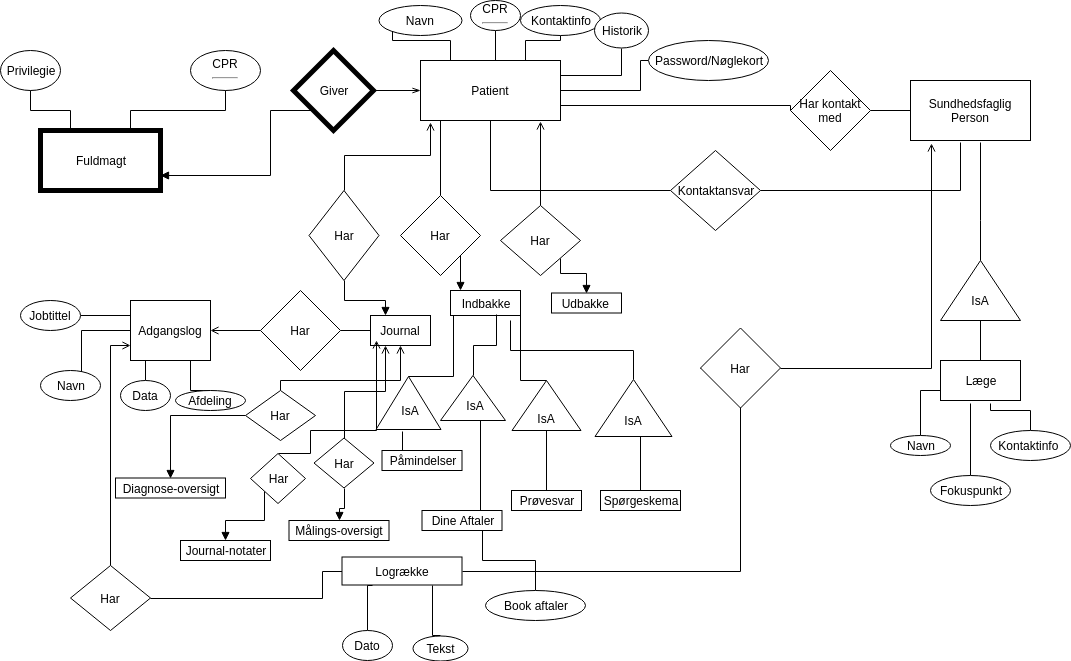
\includegraphics[width=\linewidth]{Materials/ER-diagram.png}
  \caption{ER-diagram for Min Sundhedsplatform}
  \label{fig:ER}
\end{figure}
ER Diagrammet (Ovenstående figur \ref{fig:ER}) viser den logiske model for domænet Min Sundhedsplatform. \\
Entiteterne er de logiske enheder - dvs. aktører, objekter og begivenheder i systemet. 
Relationerne angiver hvilken type af relation, der er mellem entiteterne i systemmet.

Entiteterne angives med rektangler og en tekst typisk et navneord. Til entiteterne er der tilknyttet et eller flere attributter, angivet med en ellipse med en tekst.

Relationerne angives med en diamant med en  tekst, der beskriver relationen mellem to eller flere entiteter.

kardinaliteten beskrives med streger og pile mellem entiteterne. \\ 
En sort lukket pil beskriver: mange til højst en (dvs. 0 eller 1).\\
En åben pil beskriver: mange til præcis en.\\
En streg uden pil beskriver: mange til mange.

Under-entiteter repræsenteres med relationen 'ISA' i en trekant.

En svag entitet er en entitet, der for at relationen kan gælde, kræver at den udover sine egne attributter også skal have sin ejers nøgleattribut som nøgle. Den beskrives med en fed ramme.

Vi kan læse følgende information om Min Sundhedsplatform ud af ER Diagrammet:\\
En patient har tilknyttet attributterne: navn, cpr-nummer, kontakt-info, historik og password/nøglekort. Cpr-nummer er nøgleattribut.\\
Der er en giver-relation fra entiteten patient til entiteten fuldmagt. Der er en mange til en relation, fordi patienten giver fuldmagter og fuldmagterne er givet af én patient. Fuldmagt er en svag entitet, fordi den kræver sin ejers nøgleattribut - dvs. patientens cpr-nummer som nøgleattribut. \\
Patienter har kontakt med mange sundhedsfaglige personer og mange  sundhedsfaglige personer har kontakt ansvar med mange patienter. Læger er under-entitet af sundhedsfaglig personale. \\
Patienten har højest én udbakke, og udbakken tilhører præcis en patient.\\
Patienten har højest én indbakke. Indbakke kan være Påmindelser, Dine Aftaler, Prøvesvar og Spørgeskema.\\
Patienten har højest én journal og en journal tilhører præcis en patient. \\
Journalen har præcis én adgangslog, som har mange logrækker. Logrækken har præcis en adgangslog og præcis en sundhedsfaglig person. En sundhedsfaglig person har mange logrækker.\\
Journalen har én eller ingen diagnose-oversigt og diagnose oversigten tilhører præcis en journal.\\
Journalen har enten ingen eller en journal-notater som tilhører præcis én journal.\\
Journalen har enten én eller ingen målings-oversigt som tilhører præcis én journal.

I designfasen kan den logiske model af ER diagrammet bruges til at danne et overblik over hvilke data, der skal gemmes i systemet, og hvordan flowet er (relationerne mellem entiteterne).\\
ER-diagrammet kan bruges i kommunikationen mellem it-designeren, kunden og brugerne omkring afklaringen af hvilke data, der skal indgå i systemet/domænet. \\
I udviklingsfasen kan ER-diagrammet transformeres til den fysiske model hvor man, ud fra entiteterne, opstiller databaserne/tabeller med de attributter/data, der er behov for i domænet.

        \end{document}
